% Chapter 5

\chapter{Performance Study and Particle Identification}
\label{ch:PID} % For referencing the chapter elsewhere, use \autoref{ch:name}

%----------------------------------------------------------------------------------------

For particle tracks with a measured momentum using the RICH information enables us to determine the particle mass and thus identify the particle. As the detector efficiency is not perfect, the misidentification probability is not zero ; one thus has to determine the identification performance of the RICH detector. The RICH performance study relies on extracting the identification and misidentification probabilities for pions, kaons and protons. From samples of pure pions, kaons and protons the RICH detector response is measured : the hadrons are identified using RICH information and the identification and misidentification probabilities are calculated in the hadron ($p_h$,$\theta_h$) phase space for pions, kaons and protons. The method used for identification is a likelihood estimation for different hypotheses. At first order, the mass assignment corresponds to the highest likelihood, but further requirements can be added to improve the result.

\section{Determination of RICH Detector Performance}

The identification and misidentification efficiency is given by the ratio of the number of particles correctly and wrongly identified respectively, out of pure sample of specific hadron type species over the total number of hadrons composing the pure sample :

\begin{equation}
    P(t \rightarrow i) = \frac{N(t \rightarrow i)}{N(t)}
\end{equation}

$P(t \rightarrow i)$ is the probability that a particle $t$ is identified as a particle $i$, $N(t \rightarrow i)$ is the number of particles $t$ identified as $i$ and $N(t)$ is the total number of hadron $t$ of the pure sample. The identification ($P(t \rightarrow t)$) and misidentification ($P(t \rightarrow i)$) efficiencies are properties of the RICH and can be displayed in an efficiency matrix with the identification efficiencies on the diagonal and the misidentification ones off-diagonal :

\begin{equation}
  M_R
  =
  \begin{bmatrix}
  \epsilon(\pi \rightarrow \pi) & \epsilon(K \rightarrow \pi) & \epsilon(p \rightarrow \pi)\\
  \epsilon(\pi \rightarrow K) & \epsilon(K \rightarrow K) & \epsilon(p \rightarrow K) \\
  \epsilon(\pi \rightarrow p) & \epsilon(K \rightarrow p) & \epsilon(p \rightarrow p)
  \end{bmatrix}.
\end{equation}

\subsection{Selection of $\Phi$, $K^0$ and $\Lambda$}

To obtain the efficiency matrix, three pure hadron samples are needed. The RICH performance analysis is based on the study of the pion, kaon and proton samples originating from $\Phi$, $K^0$ and $\Lambda$ decays.

For the determination of the RICH efficiency, it is necessary to have a source of events where the true kind of the particle passing the RICH is known. That kind of events is obtained using two body particle decays, namely the decay of a $K^0$ into two pions ($K^0 \rightarrow \pi^+\pi^-$), the $\Phi$ decay into two kaons ($\Phi \rightarrow K^+K^-$), the $\Lambda$ decay into a pion and a proton ($\Lambda \rightarrow p\pi^-$). In order to select events with such decays, scattering events with a scattered muon are selected. The typical cuts are thus applied to the data:
\begin{itemize}
  \item Exclude bad spills
  \item Select best primary vertex with incoming and scattered muon
  \item Check if primary vertex is inside one of the target cells
  \item Extrapolated track of the incoming muon should cross all target cells
  \item $0.1 \le y \le 0.9$
\end{itemize}

Different selection criteria have to be used for $K^0$, $\Lambda$ and $\Phi$ decays. In the case of $K^0$ mesons and $\Lambda$ baryons, the particles decay by the weak force. Therefore, the decay length is long enough to produce a secondary vertex, which can be separated from the primary one. The $\Phi$ mesons decays by the strong force. This results in a very short decay length and it is not possible to separate the secondary vertex from the primary one.

\subsection{$K^0$ and $\Lambda$ selection}

For $K^0$ mesons the decay into $\pi^+$ and $\pi^-$ with a branching ration of ($69.20$~$\pm$~$0.05$)\% \cite{PDG} and in the case of $\Lambda$ and $\bar{\Lambda}$ baryons the decay into a proton and a pion with a branching ratio of ($63.9$~$\pm$~$0.5$)\% \cite{PDG} is used. In both decays the reconstruction of the secondary vertex is possible. The following cuts are applied to select these decays:

\begin{enumerate}
  \item Selection of good secondary vertices
  \begin{itemize}
    \item Loop over all vertices
    \item Vertex is not primary one
    \item Exactly two opposite charged outgoing particles
    \item The tracks should not be connected to any other primary vertex to ensure that they belong to a secondary vertex
    \item Primary and secondary vertex separated by more than two times the reconstruction accuracy
  \end{itemize}
  \item Select good hadron tracks
  \begin{itemize}
    \item Both particles should not have crossed more than $10$ radiation length in order to supress the muons from the sample.
    \item Last measured position ($Z_{last}$) behind SM$1$ to ensure a measured momentum
    \item Transverse momentum with respect to the mother particle larger than $23$ MeV to suppress electrons from photon conversion
    \item Check that the decaying particle is connected to the primary vertex ($\theta_p \le 0.01$)
  \end{itemize}
  \item Additional cuts
  \begin{itemize}
    \item $p_h \geq 1$ GeV/$c$
    \item Mass difference smaller than $150$ MeV/$c^2$ between the $K^0$/$\Lambda$ mass and the invariant mass of the two decay hadrons assuming the correct masses
  \end{itemize}
\end{enumerate}

The same cuts except for the mass cuts are used for $K^0$ and $\Lambda$ candidates. The transverse momentum of K, $\Lambda$ or dacay product is shown as a function of the ratio of the longitudinal momentum ratio of two particles :
%
\begin{equation}
  \alpha = \frac{p_{L,1}-p_{L,2}}{p_{L,1}+p_{L,2}},
\end{equation}
%
in the Armenteros plots in Fig.~\ref{pic:Armenteros} (a) for $K^0$ and $\Lambda$ and (b) for $\Phi$.

\begin{figure}[!h]
  \centering
	\subfloat[$K^0$ and $\Lambda$]{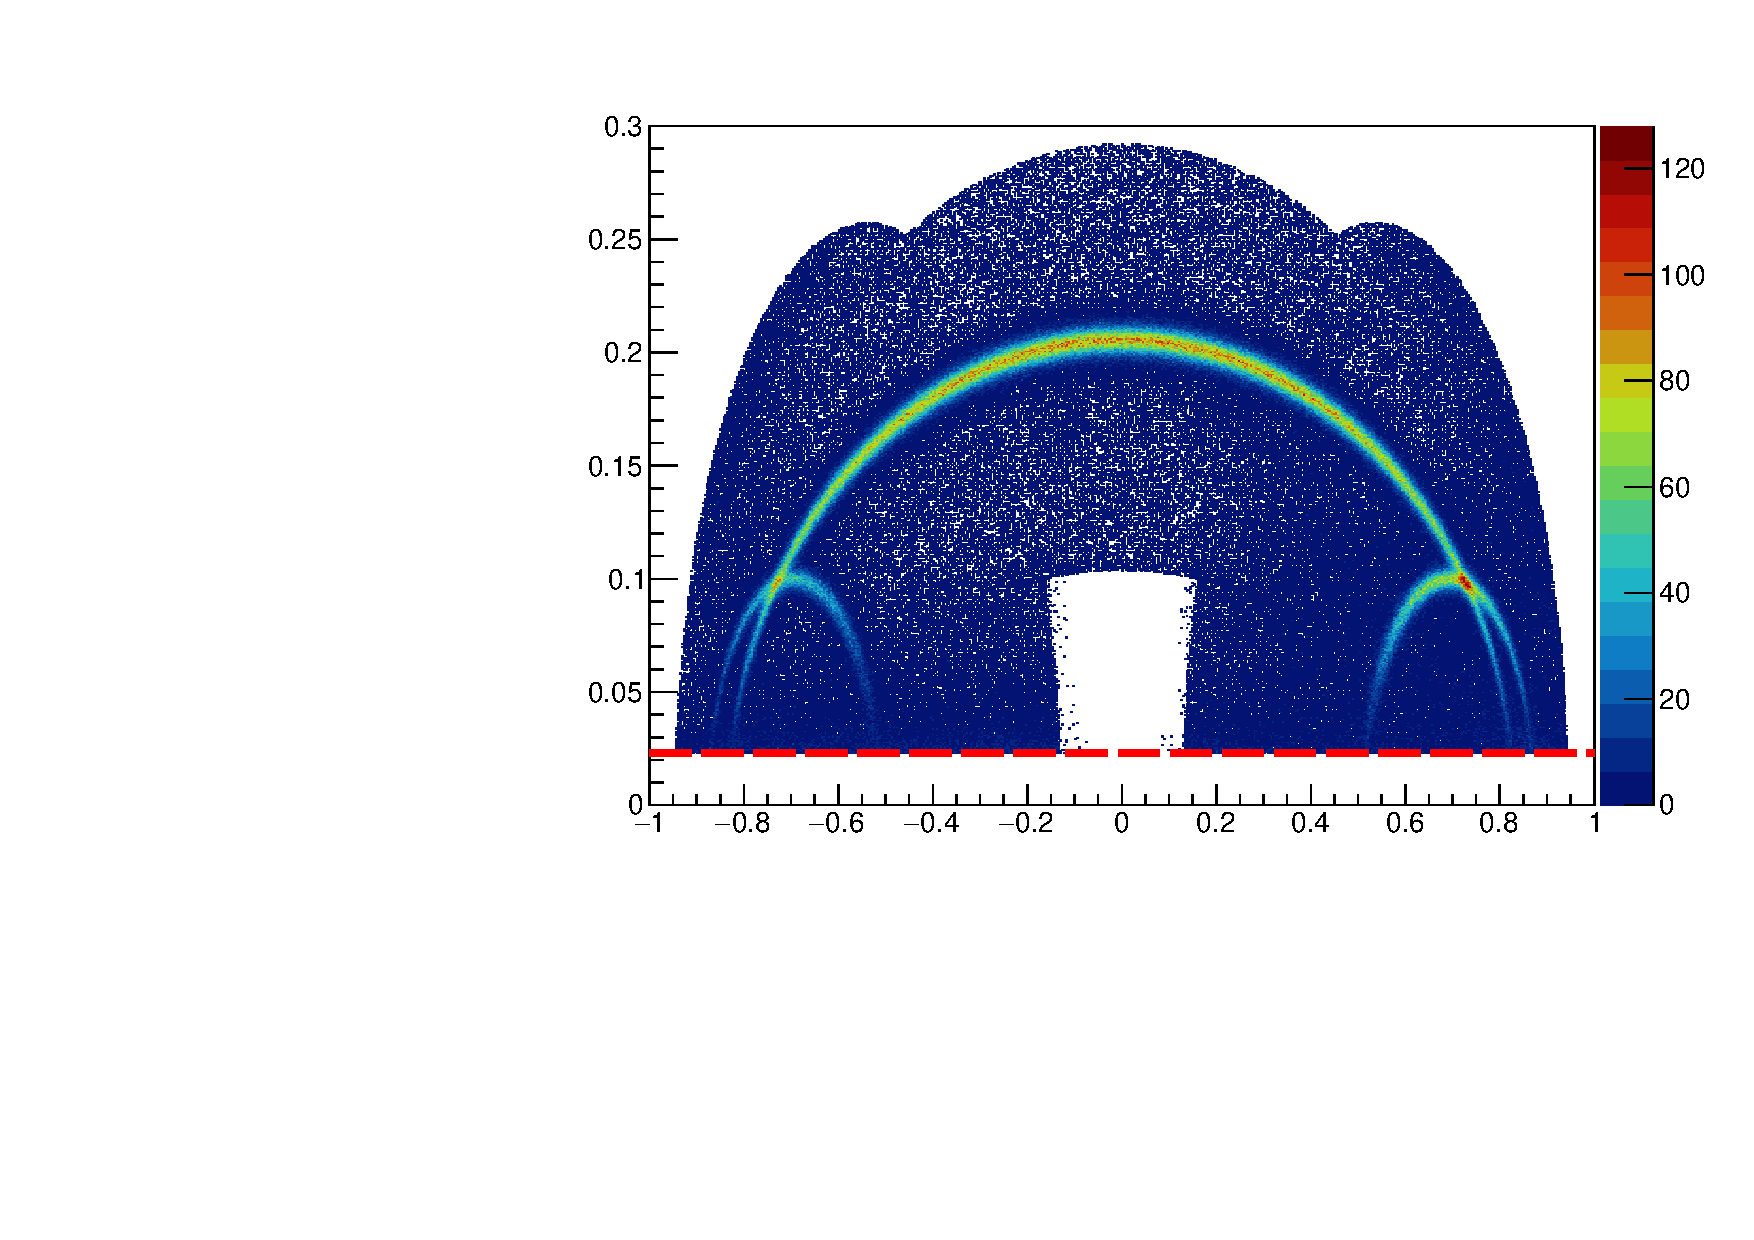
\includegraphics[scale=0.42]{./gfx/ArmenterosK0L.pdf}}
  \subfloat[$\Phi$]{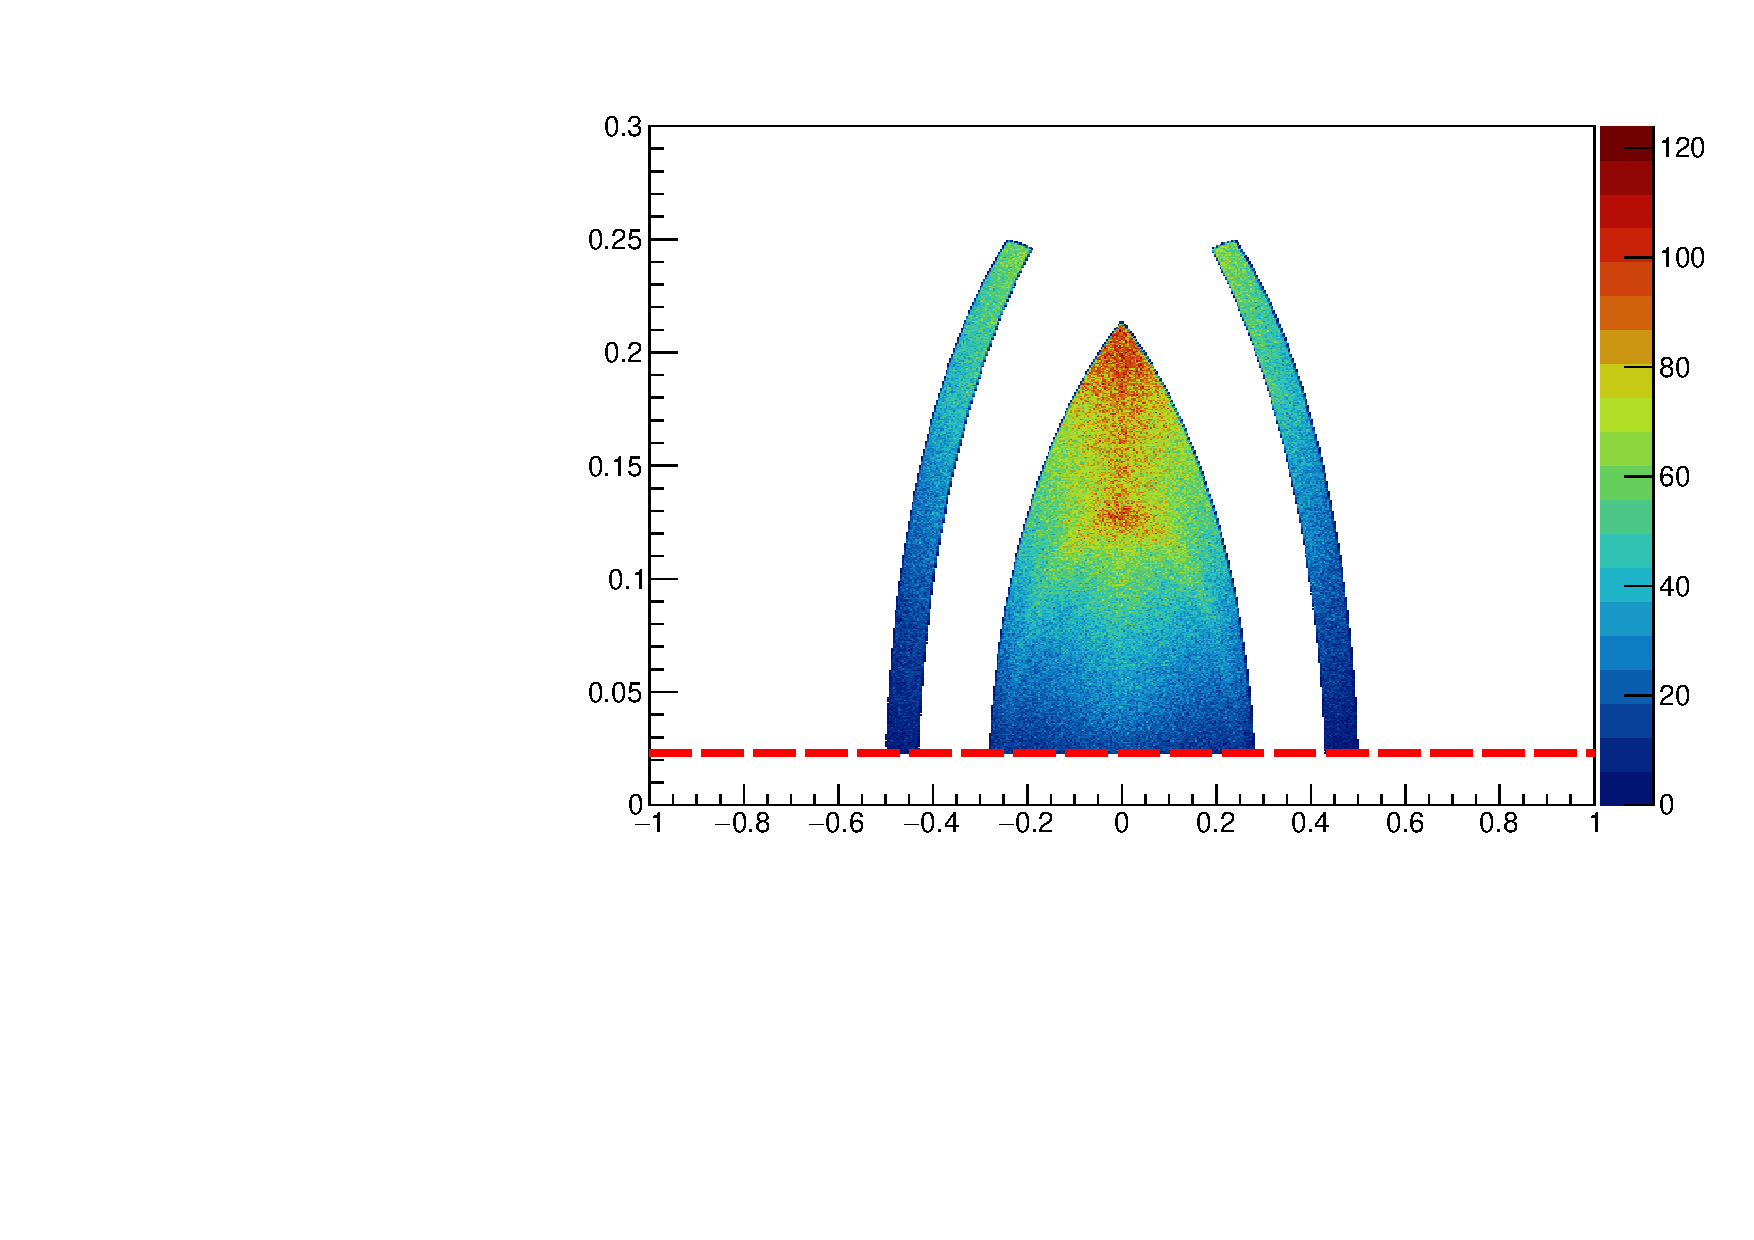
\includegraphics[scale=0.42]{./gfx/ArmenterosPhi.pdf}}
	\caption{Armenteros plots. The cut on the transverse momemtum is illustrated by the red line.}
	\label{pic:Armenteros}
\end{figure}

The three visible arcs are produced by the decay of the $K^0$ mesons and the $\Lambda$ baryons. The decay of $K^0$ mesons in two particles with the same mass results in the symmetric arc, whereas the decay of $\Lambda$ baryons into two particles with different masses result in the two smaller arcs on the left and right side. All particles below the red dashed line, which corresponds to the $23$ MeV limit, are rejected in order to supress tracks from electron coming from photon conversion.

\subsection{$\Phi$ selection}

The branching ratio of the $\Phi$ decay into two kaons is ($48.9$~$\pm$~$0.5$)\% \cite{PDG}. The $\Phi$ meson decay length is too short to separate the primary and decay vertex. Therefore, all outgoing particles from a primary vertex are taken into account for the search of possible $\Phi$ mesons. The selection steps are similar the selection of the $K^0$/$\Lambda$ candidates :

\begin{enumerate}
  \item Selection of possible good events with $\Phi$ mesons
  \begin{itemize}
    \item At least three outgoing particles including scattered muon
    \item Loop over all outgoing particles
    \item Oppositely charged pairs of hadrons (none is a muon)
  \end{itemize}
  \item Select good hadron tracks
  \begin{itemize}
    \item Last measured position ($Z_{last}$) behind SM1 to ensure a measured momentum
    \item Transverse momentum with respect to the mother particle larger than $23$ MeV to suppress electrons from photon conversion
  \end{itemize}
  \item Additional cuts
  \begin{itemize}
    \item $9$ GeV/$c$ $\leq p_h \leq 55$ GeV/$c$
    \item Mass difference smaller than $120$ MeV/c$^2$ between the $\Phi$ mass and the invariant mass of the two decay hadrons assuming the kaon mass.
  \end{itemize}
\end{enumerate}

The selection of $\Phi$ meson candidates results in a large combinatorial background.

\section{Likelihood method}

The likelihood (LH) method is a statistical method that can be used to find a suitable model for describing a data set or to estimate the values of the parameters used in this model \cite{LH1,LH2}.

The first step is to define the LH function. With a sample $\mathbf{s}$ of elements $s_i$, $i \in \llbracket 1,l \rrbracket$ :
%
\begin{equation}
  \mathbf{s} = \left( s_1,s_2,..,s_l \right),
\end{equation}
%
which follows a distribution with the probability density $f(s|\theta)$. This probabilty density is determined by a set of parameters $\theta = \theta_1,..,\theta_m$. In order to fit the sample with the model some requirements must be met.

\begin{enumerate}
  \item The sample can be considered as a $l$-dimensional random variable and can be assigned a probability density $g(\mathbf{s})$ :
  \begin{equation}
    g(\mathbf{s}) = g\left( s_1,s_2,..,s_l \right).
  \end{equation}
  \item The sample is random.
  \begin{enumerate}[(a)]
    \item The $s_i$ are independent :
    \begin{equation}
      g(\mathbf{s}) = g_1\left(s_1 \right) \cdot g_2\left(s_2 \right) \cdot .. \cdot g_l\left(s_l \right).
    \end{equation}
    \item Each element $s_i$ follows the probability density of the distribution :
    \begin{equation}
      g(s_i) = f(s|\theta).
    \end{equation}
  \end{enumerate}
\end{enumerate}

If these conditions are fulfilled, the LH function $L\left(s_1,..,s_l|\theta \right)$ is defined as :
%
\begin{equation}
  L\left(s_1,..,s_l|\theta \right) = \prod_{i=1}^{l} f(s_i|\theta),
\end{equation}
%
and states that the probability of occurence of the sample is equal to the product of the occurence of each element of the sample. The probability density of the sample is normalized to its domain of definition $\Omega$ :
%
\begin{equation}
  \int_{\Omega} L\left(s_1,..,s_l|\theta \right) ds_1 .. ds_l = 1.
\end{equation}
%
In order to select from all possible sets of parameters in $\Theta$ the estimator $\hat{\theta}$, which gives the best description of the true description, one applies the Maximum Likelihood Estimation (MLE) method. The method can be formulated as follows :
%
\begin{equation}
  \hat{\theta} \in \left \{ \underset{\theta \in \Theta}{arg\,max}\,L\left(s_1,..,s_l|\theta \right) \right \},
\end{equation}
%
if a maximum exists. This means that the maximum of the LH function has to be found in relation to the parameters. Having found the maximum, one has also found the best estimate of the parameters. Since the LH function can yield very small values as a probability density, it is common to defin the logarithmic LH function instead :
%
\begin{equation}
  \mathscr{L}\left(s_1,..,s_l|\theta \right) = \text{ln}\,L\left(s_1,..,s_l|\theta \right) = \sum_{i=1}^{l} \text{ln}\,f(s_i|\theta).
\end{equation}
%
The maximization condition for several parameters $\theta = \theta_1,..,\theta_m$ is thus :
%
\begin{equation}\label{eq:maximization}
  \frac{\delta \mathscr{L}\left(s_1,..,s_l|\delta\theta \right)}{\delta\theta_j} = \frac{\delta}{\delta\theta_j} \sum_{i=1}^{l} \text{ln}\,f(s_i|\theta) = 0 \quad for \quad \theta = \hat{\theta}.
\end{equation}
%
In many physics systems one can find geometrical or kinematic constraints such as the sum of the impulses equal to zero and the sum of the energies equal to twice the photon energy in the electron-positron annihilation in the center-of-mass system. These conditions can be used to eliminate one of the parameters of the system. However, this is often not desirable since this elimination is often only possible through complicated algorithm or the equivalent treatment of the parameters after the adaptation is no longer guaranteed. In order to consider the constraints further, they can be included in the LH functions as functions $c_{k}(\theta)(k=1,..,z_c)$, analogous to the method of Lagrange multipliers :
%
\begin{equation}
  \mathscr{L}\left(s_1,..,s_l|\delta\theta \right) = \text{ln}\, L\left(s_1,..,s_l|\theta \right) = \sum_{i=1}^{l} \text{ln}\, f(s_i|\theta) - \sum_{k=1}^{z_{c}} \lambda_k c_k(\theta)
\end{equation}
%
The overall $z_c$ Lagrange multipliers $\lambda_k$ are treated as additional parameters. Thus the $z_c$ conditions of the constraints still come to the maximization conditions in Eq.~\ref{eq:maximization} :
%
\begin{equation}
  \frac{\delta \mathscr{L}}{\delta \lambda_k} = c_k(\theta) = 0.
\end{equation}
%
Since the LH method is used not only for particle identification by the RICH detector but also for the fits to determine the RICH efficiencies, the extended Maximum Likelihood Estimation (eMLE) method is discussed further below. This method is used primarily for problems in which the fit also supplies the number of expected events and these are to be adapted to the observed events. For example this is the case if there are $n$ events that results from a sum of several sources $n_i$. The constraint that follows is that $n = \sum_{i=1}^{j} n_i$. This condition can now be used as an additional factor in the LH function. The factor then corresponds to a Poisson distribution, which describes the probability that $n$ events are also observed at an expected value $\lambda$ :
%
\begin{equation}
  L\left(s_1,..,s_l|\theta \right) = \frac{\lambda^n e^{-\lambda}}{n!} \prod_{i=1}^{n} f(s_i|\theta).
\end{equation}
%
For the logarithmic LH function follows :
%
\begin{equation}\label{eq:loglambda}
  \mathscr{L}\left(s_1,..,s_l|\theta \right) = n \,\text{ln}\, \lambda - \lambda + \sum_{i=1}^{n} \text{ln},f(s_i|\theta)
\end{equation}
%
The term $- \text{ln} n!$ is irrelevant for the following maximization and has been omitted. With the help of the following simplification :
%
\begin{equation}
  n \,\text{ln}\, \lambda + \sum_{i=1}^{n} \text{ln}\, f(s_i|\theta) =  \sum_{i=1}^{n} \left(\text{ln}\, f(s_i|\theta) + \text{ln}\, \lambda \right) = \sum_{i=1}^{n} \text{ln}\, (\lambda f(s_i|\theta)),
\end{equation}
%
is it possible to define a function $g(s_i|\theta) = \lambda f(s_i|\theta)$, which is normalized by $\lambda$ :
%
\begin{equation}
  \int_{\Omega} g(s_i|\theta) ds_1 .. ds_l = \lambda \int_{\Omega} f(s_i|\theta)ds_1 .. ds_l  = \lambda.
\end{equation}
%
Thus Eq.~\ref{eq:loglambda} can be rewritten into the common form of extended LH function :
%
\begin{equation}
  \mathscr{L}\left(s_1,..,s_l|\theta \right) = \sum_{i=1}^{n} \text{ln}\, g(s_i|\theta) - \int_{\Omega} g(s_i|\theta) ds_1 .. ds_l.
\end{equation}
%
It follows that $\mathscr{L}\left(s_1,..,s_l|\theta \right)$ becomes maximal when the additional term equals the number of actual events $n$.

\section{RICH Particle Identification}

Particle identification using the LH method is accomplished by finding the maximum LH function value. The LH function describes the radial photon distribution. An essential step is to determine the radial photon distribution (see Fig.~\ref{pic:Photonfit} (a)) as precisely as possible. This depends on the detector geometry, the accuracy in determining the trajectory of the particle to be identified, as well as on the accuracy with which the parameters describing the photon position in the ring plane can be determined. The two parameters used are the reconstructed angles at which the photon ($Ph$) was emitted relative to the particle path $\Theta^{Ph}$ and the reconstructed azimuthal angle around the particle path $\Phi^{Ph}$ \cite{Pfit1,Pfit2,Pfit3}. The LH function for describing the photon distribution is given as:
%
\begin{equation}
  L_{N_{Ph}} = \prod_{k=1}^{N_{Ph}} \left[ (1-\epsilon) G\left(\Theta_k^{Ph},\Phi_k^{Ph} \right) + \epsilon B\left(\Theta_k^{Ph} \right) \right],
\end{equation}
%
where
%
\begin{equation}
  G\left(\Theta_k^{Ph},\Phi_k^{Ph} \right) = \frac{1}{\sqrt{2\pi} \cdot \sigma_{\theta,k}^{Ph}} e^{-\frac{1}{2}\frac{\left(\Theta_k^{Ph}-\Theta_k^{Ph} \right)^2}{\left(\sigma_{\theta,k}^{Ph} \right)^2}} \cdot \frac{\Theta_k^{Ph}}{\Theta^{M}}
\end{equation}
%
is a Gaussian distribution with which the signal (see Fig.~\ref{pic:Photonfit} (b)) can be described. The standard deviation $\sigma_{\theta}^{Ph}(\Phi_P^{Ph},\beta)$ originates from the accuracy with which the photon distribution can be determined. This in turn depends on the azimuthal photon angle ($\Phi_P^{Ph}$) in the plane of the photodetectors, which is characterized by the index $P$, and on the particle velocity relative to the speed of light $\beta$. $\Theta^M$ is the mass hypothesis is designated. It is determined by the expected Cherenkov angle for a particular particle type or particle mass with $\beta$. Possible particles are electrons, pions, kaons and protons.

\begin{figure}[!h]
  \centering
	\subfloat[Photon distribution in the detector plane]{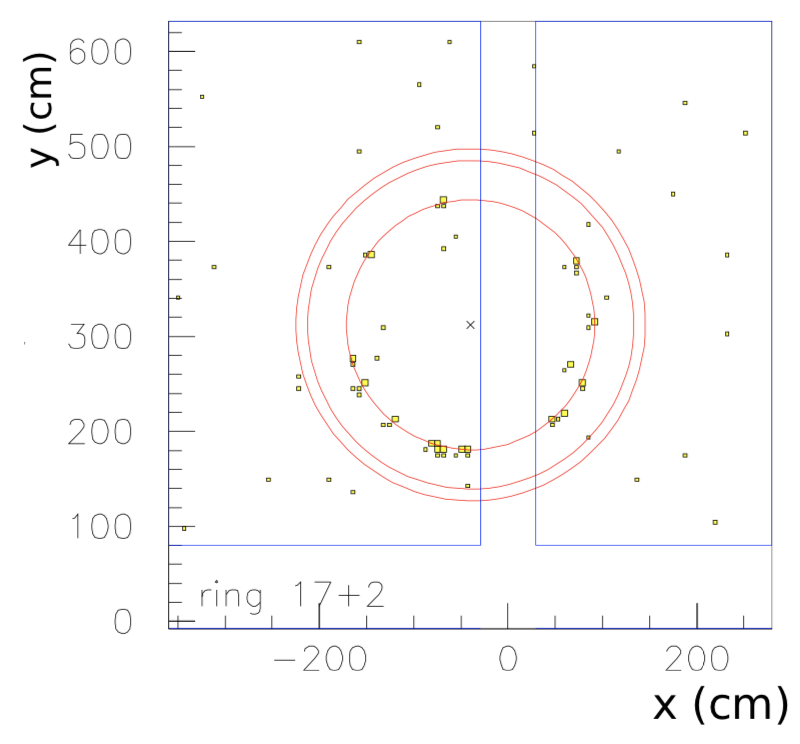
\includegraphics[scale=0.52]{./gfx/LH1.png}}
  \subfloat[LH-fit of the radial photon distribution]{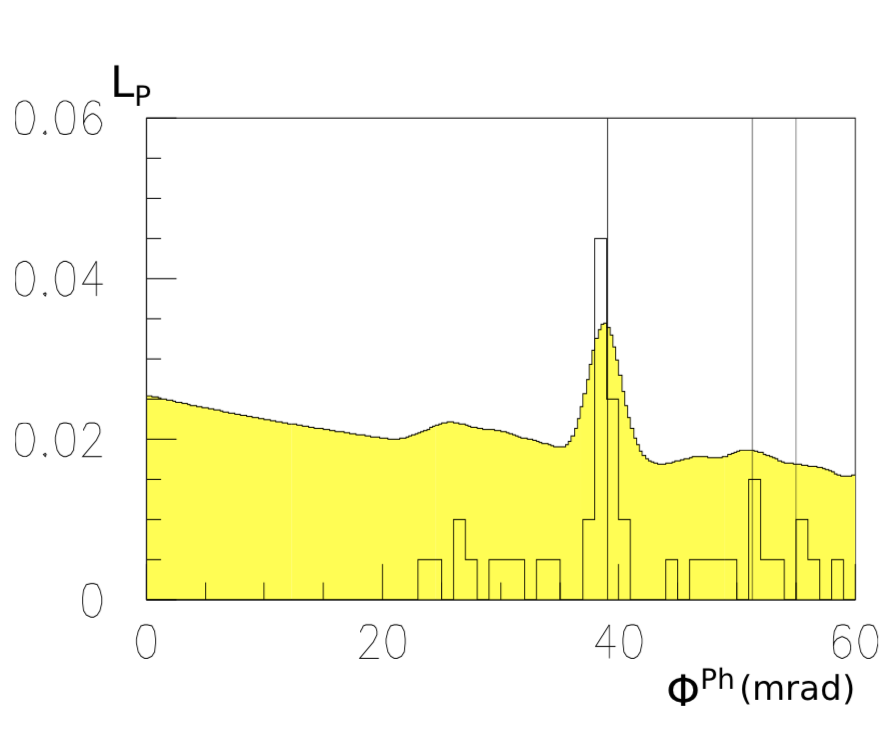
\includegraphics[scale=0.52]{./gfx/LH2.png}}
	\caption{Figure (a) shows the photon distribution in the plane of the photodetectors. The x marks the projection of the particle path. The red rings correspond, from the inside to the outside, to the distribution that would be generated by a proton, a kaon or a pion. The yellow marks are the detected photons. In (b) the result of the LH-fit of the photon distribution with the proton hypothesis is shown.}
	\label{pic:Photonfit}
\end{figure}

The goal of the selection is a clean pion and kaon sample. The RICH particle identification efficiency is studied in the momentum range of $3$ GeV/$c$ $ \leq p \leq $ $50$ GeV/$c$. In this range, pions and kaons are emitting Cherenkov light, while up to $\sim$ $17$ GeV protons are still below the threshold of :
%
\begin{equation}
  p_{thr,i} = \frac{m_i}{ \sqrt{n^{2}-1} }
\end{equation}
%
where $n$ is the refractive index. This is shown in Fig.~\ref{pic:RefIndex} where the reconstructed Cherenkov angle is shown as a function of the hadron momentum. The identification of pions, kaons and protons above the momentum threshold is done by comparing the likelihood values with one another. The identification of these particles is done using likelihood cuts. Using the likelihood values, the particle identification is done by comparing these values with one another. In the simplest case, the highest one determines the particle type. This method is used in the case of pions. In the case of kaons, stricter likelihood cuts are applied to suppress misidentified pions. Due to the larger amount of pions compared to kaons stricter selection cuts are imposed for kaons. The likelihood cuts for protons require its likelihood to be the largest one.  Below the momentum threshold, protons do not emit Cherenkov light. Therefore, the likelihood values are used to test whether the detected light is consistent with random noise in the detector (background). In order to avoid possible problems due to the uncertainty on the reconstructed momentum or the uncertainty of the refractive index of the RICH gas, a region of $\pm$ $5$ GeV/$c$ around the proton threshold is used, where both hypothesis are applied for proton identification. The likelihood cuts are listed in Table.~\ref{tab:LHcut}. As the electrons cannot be distinguished from pions for momentum above $8$ GeV, they are not separated at this stage of the analysis. This contamination is dealt with the Monte-Carlo later in the analysis (Chapter~\ref{ch:CF}).

\begin{table}[!h]
  \caption{Likelihood cuts for pion, kaon and protons}
  \label{tab:LHcut}
  \centering
  \begin{tabular}{lccccc}
    \hline
     & PION & KAON & \multicolumn{3}{c}{PROTON} \\
    \hline
    MOMENTUM & $p$ > $p_{\pi,thr}$ & $p$ > $p_{K,thr}$ & \multicolumn{2}{c}{$p$ $\leq$ $p_{p,thr}$} & $p$ > $p_{p,thr}$ \\
     & $\pi$ & $K$ & $p$ & $\bar{p}$ & $p/\bar{p}$ \\
    LH($\pi$)/LH($2^{nd}$) & $> 1.02$ & --- & --- & --- & --- \\
    LH($\pi$)/LH(bg) & $> 2.02$ & --- & $< 2.2$ & $< 2.1$ & $< 1.$\\
    LH($K$)/LH($2^{nd}$) & --- & $> 1.08$ & --- & --- & --- \\
    LH($K$)/LH(bg) & --- & $> 2.08$ & $< 2.9$ & $< 2.8$ & $< 1.$ \\
    \hline
  \end{tabular}
\end{table}

\begin{figure}[!h]
  \centering
	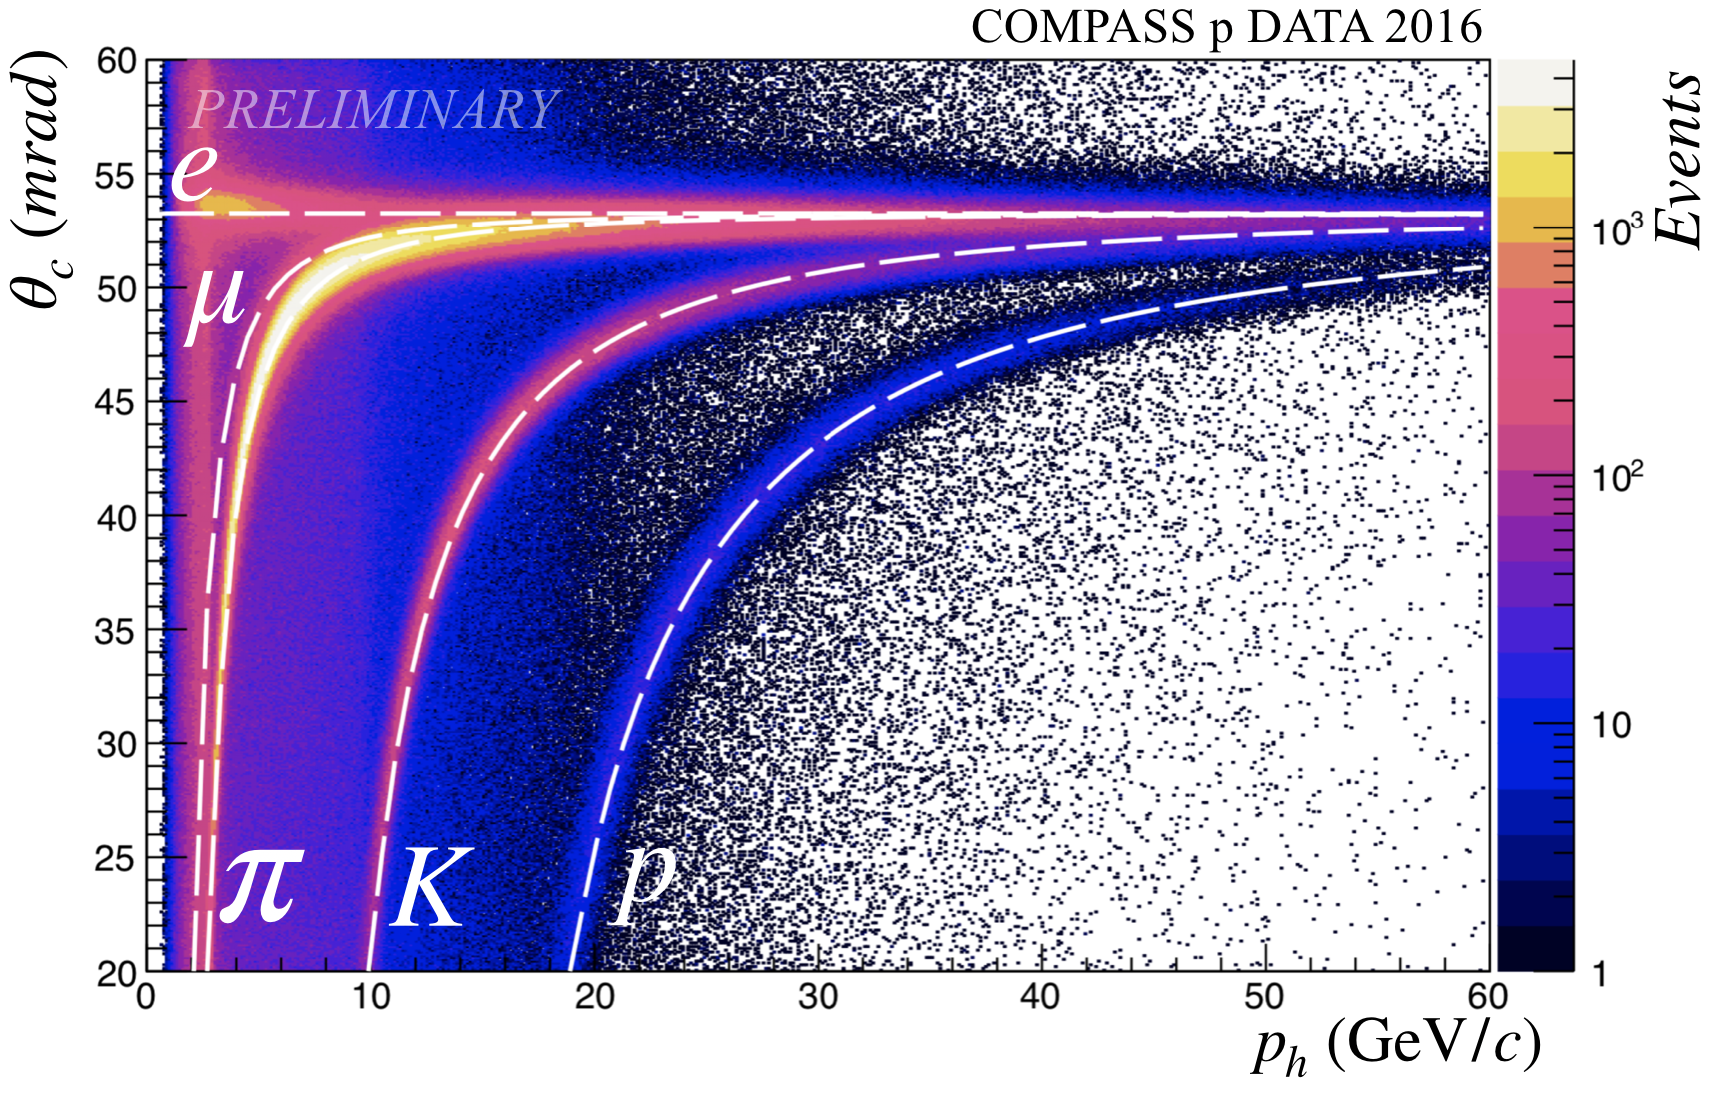
\includegraphics[scale=0.45]{./gfx/RICHIndices.png}
	\caption{Comparison of reconstructed Cherenkov angle as a function of the momentum with the calculated Cherenkov angle for each particle type using the refractive index of the RICH gas. This plot is not used for the PID.}
	\label{pic:RefIndex}
\end{figure}

\section{Method of unfolding}

The particle identification efficiency of the RICH is studied as a function of the hadron phase space. Here we use the hadron momentum and the polar angle at the entrance of the RICH, as already studied before, for example in Reference \cite{Curiel}. A fine binning is used for the momentum dependence, since the Cherenkov effect depends strongly on this variable. For the dependence on the polar angle, a coarse binning can be used, since only a weak dependence is observed. The binning used is:

\begin{itemize}
  \item Momentum $p_h$ (GeV/$c$) : \{$3,5,7,10,12,13,15,17,19,22,25,27,30,35,40,50$\}
  \item Angle $\theta_h$ (rad) : \{$0,0.01,0.04,0.12,0.3$\}
\end{itemize}

For each bin, the elements of the efficiency matrix $M_R$ are determined separately for positive and negative particles. The elements of this matrix contain the probability for a particle $t$ to be identified as a particle of type $i$, for example a pion that is correctly identified as pion or wrongly as a kaon. The full matrix is given by:

\begin{equation}
  M_R
  =
  \begin{bmatrix}
  \epsilon(\pi \rightarrow \pi) & \epsilon(K \rightarrow \pi) & \epsilon(p \rightarrow \pi)\\
  \epsilon(\pi \rightarrow K) & \epsilon(K \rightarrow K) & \epsilon(p \rightarrow K) \\
  \epsilon(\pi \rightarrow p) & \epsilon(K \rightarrow p) & \epsilon(p \rightarrow p)
  \end{bmatrix}
\end{equation}

The different elements are determined by $\varepsilon(t \rightarrow i)$ = $N(t \rightarrow i)/N(t)$ where $N(t)$ is the total number of particles $t$ and $N(t \rightarrow i)$ is the number of particles~$t$, which are identified as particle~$i$ using the clean samples described above. In the case of positive pions, the events from the $K^0$ sample are used, where the negative hadron is identified as a pion using the likelihood cuts shown in Table.~\ref{tab:LHcut}.  Therefore, the second particle has to be a pion too, if the decaying particle was a $K^0$. Using the RICH, the particle type is determined for the second particle, which  results in the number $N(\pi^+ \rightarrow i)$. An equivalent procedure is used for positive kaons and protons using the $\Phi$ and $\Lambda$ samples. In order to obtain these numbers for the negative particles, the same samples are used but this time performing the identification of the positive particle in the first place. The numbers $N(t \rightarrow i)$ are extracted using a fit, which is described here for the $K^0$ sample, where the negative pion is already identified. The events are put into five different groups, depending on the particle type determined by the RICH :

\begin{itemize}
  \item All events (RICH not used for second particle)
  \item Events where $\pi^+$ is identified as $\pi^+$
  \item Events where $\pi^+$ is identified as $K^+$
  \item Events where $\pi^+$ is identified as $p$
  \item Events where $\pi^+$ is not identified
\end{itemize}

For each of these groups, the invariant $K^0$ mass spectra are shown in Fig.~\ref{pic:K0MassSpectra}, for a selected momentum bin. The number of events in the peak and the background are determined by a simultaneous fit of all five spectra. These spectra are described using two Gaussian distributions with the same mean for the signal, $f_{sig}$, and a polynomial to describe the background, $f_{bg}$. Their expressions are given in Table.~\ref{tab:FunctionForm}. The two Gaussian distributions account for the different resolutions of the two spectrometer stages. The fitted function for each of the groups is given by

\begin{equation}
  f(x) = N_{sig} \cdot f_{sig} + N_{bg} \cdot f_{bg}
\end{equation}

where $N_{sig}$ is the amount of $K^0$ and $N_{bgd}$ the amount of background events. Here, the same widths, $\sigma_1$ and $\sigma_2$, of the two Gaussian distributions was used for all five spectra.

\begin{table}[!h]
  \caption{Functional form for the descriptin of the mass spectra for $K^0$, $\Phi$ and $\Lambda$ candidates from the clean samples. The symbol $G$ represents a Gaussian distribution and the symbol $BW$ a relative Breit-Wigner distribution.}
  \label{tab:FunctionForm}
  \centering
  \begin{tabular}{lcc}
    \hline
    SAMPLE & SIGNAL & BACKGROUND \\
    \hline
    $K^0$ & $\delta G(\mu,\sigma_1) + (1-\delta)G(\mu,\sigma_2)$ & $1+ax+b(2x^2-1)+c(4x^3-3x)$ \\
    $\Phi$ & $BW(\mu,\sigma_1) \otimes G(\mu,\sigma_2)$ & $(x-t)^n \cdot exp(-a(x-t))$ with $t=2 \cdot m_K$ \\
    $\Lambda$ & $\delta G(\mu,\sigma_1) + (1-\delta)G(\mu,\sigma_2)$ & $(x-t)^n \cdot exp(-a(x-t))$ with $t= m_p + m_{\pi}$ \\
    \hline
  \end{tabular}
\end{table}

\begin{figure}[!h]
  \centering
	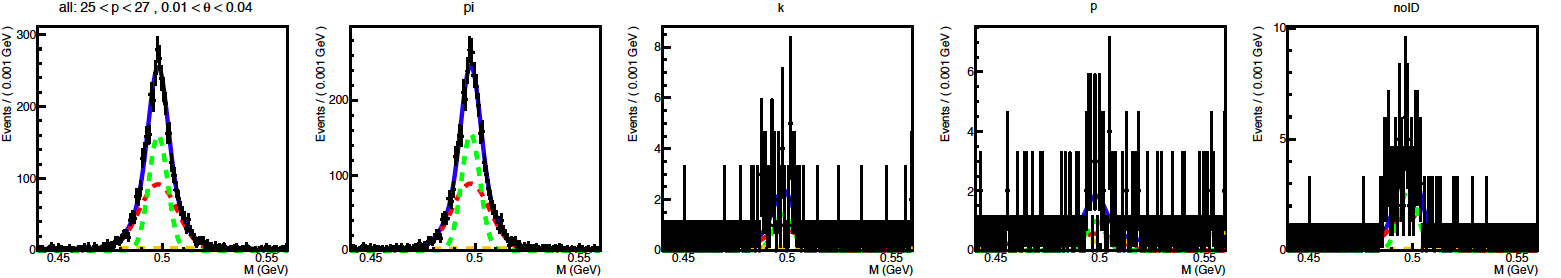
\includegraphics[scale=0.3]{./gfx/K0MassSpectra.png}
	\caption{Mass spectra for $K^0$ candidates with an identified $\pi^-$ for various hypotheses for the second hadron (from left to right : all, $\pi$, $K$, $p$, no ID). The momentum of the positive hadron is in the range of [$25$,$27$] GeV/$c$ and in the angle in the range [$0.01$,$0.04$] rad.}
	\label{pic:K0MassSpectra}
\end{figure}

Also the ratio $\delta$ of the amount of events in both Gaussian distributions is assumed to be the same. The shape of the background is the same for all spectra, except for the one where the pion is identified as a proton. In this case, a possible background contribution due to decays from $\Lambda$ baryons into a pion and an proton can be found. This results in a slightly different background shape. The integral of the background remains a independent parameter in all five cases. In order to ensure that the sum of all efficiencies  ($\varepsilon(\pi^+ \rightarrow \pi^+)  + \varepsilon(\pi^+ \rightarrow K^+ ) + \varepsilon(\pi^+ \rightarrow p ) + \varepsilon(\pi^+ \rightarrow noID)$) is $100$\%, an additional constraint is introduced to the fit.

\begin{equation}
  N^{all}(K^0) = N^{\pi}(K^0) + N^{K}(K^0) + N^{p}(K^0) + N^{noID}(K^0)
\end{equation}

where $N_i(K^0)$ (i = $\pi$, $K$, $p$, $noID$) is the number of $K^0$ obtained from the histogram where the pion is identified as $i$. This results in $16$ free parameters of the fit.

The main difference between the fits of $K^0$, $\Phi$ and $\Lambda$ samples is the description of the signal and the background, while the same method is used. The functions describing both are also given in Table.~\ref{tab:FunctionForm}. Again the parameters describing the shape are the same in all five spectra and the fit parameters  describing the integrals of the functions are used as free parameters, except for the parameter of the mass spectrum including all events. This results in $15$ free parameters for the fit of the $\Phi$ sample and in $15$ free parameters for the fit of the $\Lambda$ sample. Examples of the fits performed for the $\Phi$ and $\Lambda$ samples are shown in Figs.~\ref{pic:PhiMassSpectra} and \ref{pic:LambdaMassSpectra}. The fits show the results for the same momentum bin ($25$ GeV/$c$ $<$ $p_h$ $<$ $27$ GeV/$c$) and angular bin ($0.01$ rad $< \theta <$ $0.04$ rad), which was also shown for the $K^0$ sample.

\begin{figure}[!h]
  \centering
	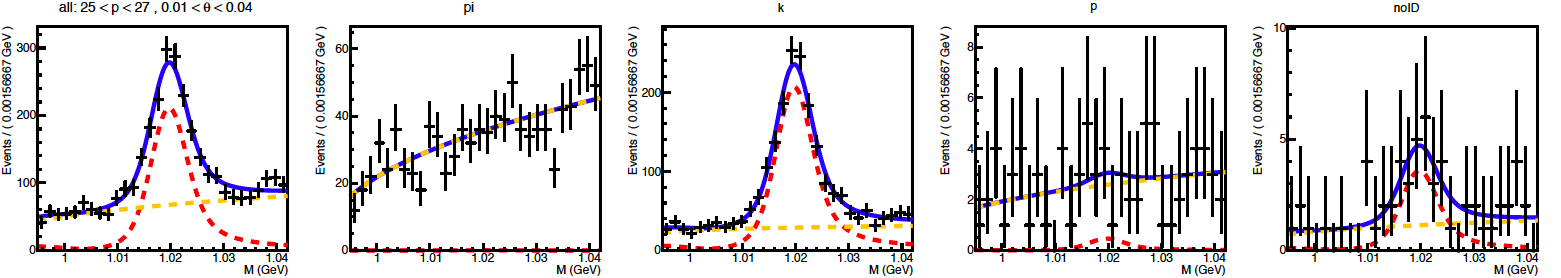
\includegraphics[scale=0.3]{./gfx/PhiMassSpectra.png}
	\caption{Mass spectra for $\Phi$ candidates with an identified $K^-$ for various hypotheses for the second hadron (from left to right : all, $\pi$, $K$, $p$, no ID). The momentum of the positive hadron is in the range of [$25$,$27$] GeV/$c^2$ and in the angle in the range [$0.01$,$0.04$] rad.}
	\label{pic:PhiMassSpectra}
\end{figure}

\begin{figure}[!h]
  \centering
	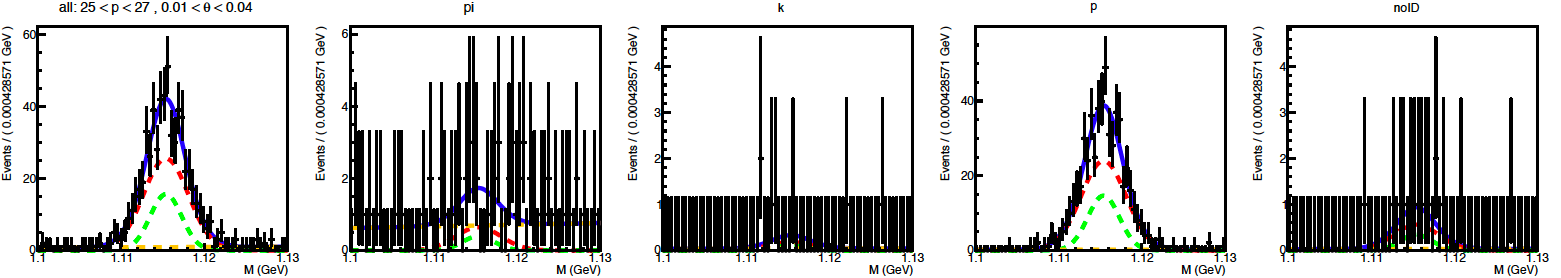
\includegraphics[scale=0.3]{./gfx/LambdaMassSpectra.png}
	\caption{Mass spectra for $\Lambda$ candidates with an identified $\pi^-$ for various hypotheses for the second hadron (from left to right : all, $\pi$, $K$, $p$, no ID). The momentum of the positive hadron is in the range of [$25$,$27$] GeV/$c^2$ and in the angle in the range [$0.01$,$0.04$] rad.}
	\label{pic:LambdaMassSpectra}
\end{figure}

\section{Calculation of the efficiencies and uncertainties}

The elements of the efficiency matrix $M_R$ are determined from fitted numbers of signal events,

\begin{equation}
  \epsilon(t\rightarrow i) = \frac{N(t\rightarrow i)}{N(t)}
\end{equation}

Here, $N(t)$ is given by the sum of all $N(t \rightarrow i)$. As the nominator and denominator are correlated, the uncertainty has to be determined via error propagation taking into account the covariance matrix of the fit,

\begin{equation}
  \Delta \epsilon = \sqrt{\sum_{j=1}^m \left( \frac{\delta \epsilon}{\delta N(i\rightarrow j)} \right)^2 \cdot u_j + 2 \sum_{j=1}^{m-1} \sum_{k=j+1}^{m} \left( \frac{\delta \epsilon}{\delta N(i\rightarrow j)} \frac{\delta \epsilon}{\delta N(i\rightarrow k)} \cdot u(j,k) \right)}
\end{equation}

where $u_j$ are the diagonal elements of the covariance matrix, $u(i,j)$ are the off diagonal elements and $\epsilon$ is one of the elements of the efficiency matrix. The summations are done over all possible particle types i.e. pion, kaon, proton and non identified.

\section{Results} \label{sec:Results}

The results for the RICH particle identification efficiency are shown in Figs. \ref{pic:Effpip} to \ref{pic:Effpm} for $\pi^+$ and $K^+$ for the various particle types and charges. The plots for the other species can be found in Appendix~\ref{ch:appRICH}. In each figure, the momentum dependence for the different angular bins is shown. The efficiencies are weakly dependent on the angle, while it is more strongly correlated with the momentum, especially in the region near the threshold.
The RICH performs a correct identification of pions in more than $95$\% of the cases for momenta below 30 GeV/$c^2$ and the probability for a misidentification of a pion as a kaon is below $\sim$ $1$\%. For kaons, near the threshold, a strong momentum dependence of the efficiencies is observed. Therefore a cut of $12$ GeV is chosen in the following analysis. At higher momenta the correct identification is given in $\sim$ $95$\% of the cases and the probability for a misidentification of a kaon as a pion is below $\sim$ $2$\%. For protons, the momentum dependence around threshold level is even stronger. Below the threshold, protons are identified correctly in $50$\% of the cases. Above the threshold numbers rise to $\sim$ $95$\%.

\begin{figure}[!p]
  \centering
	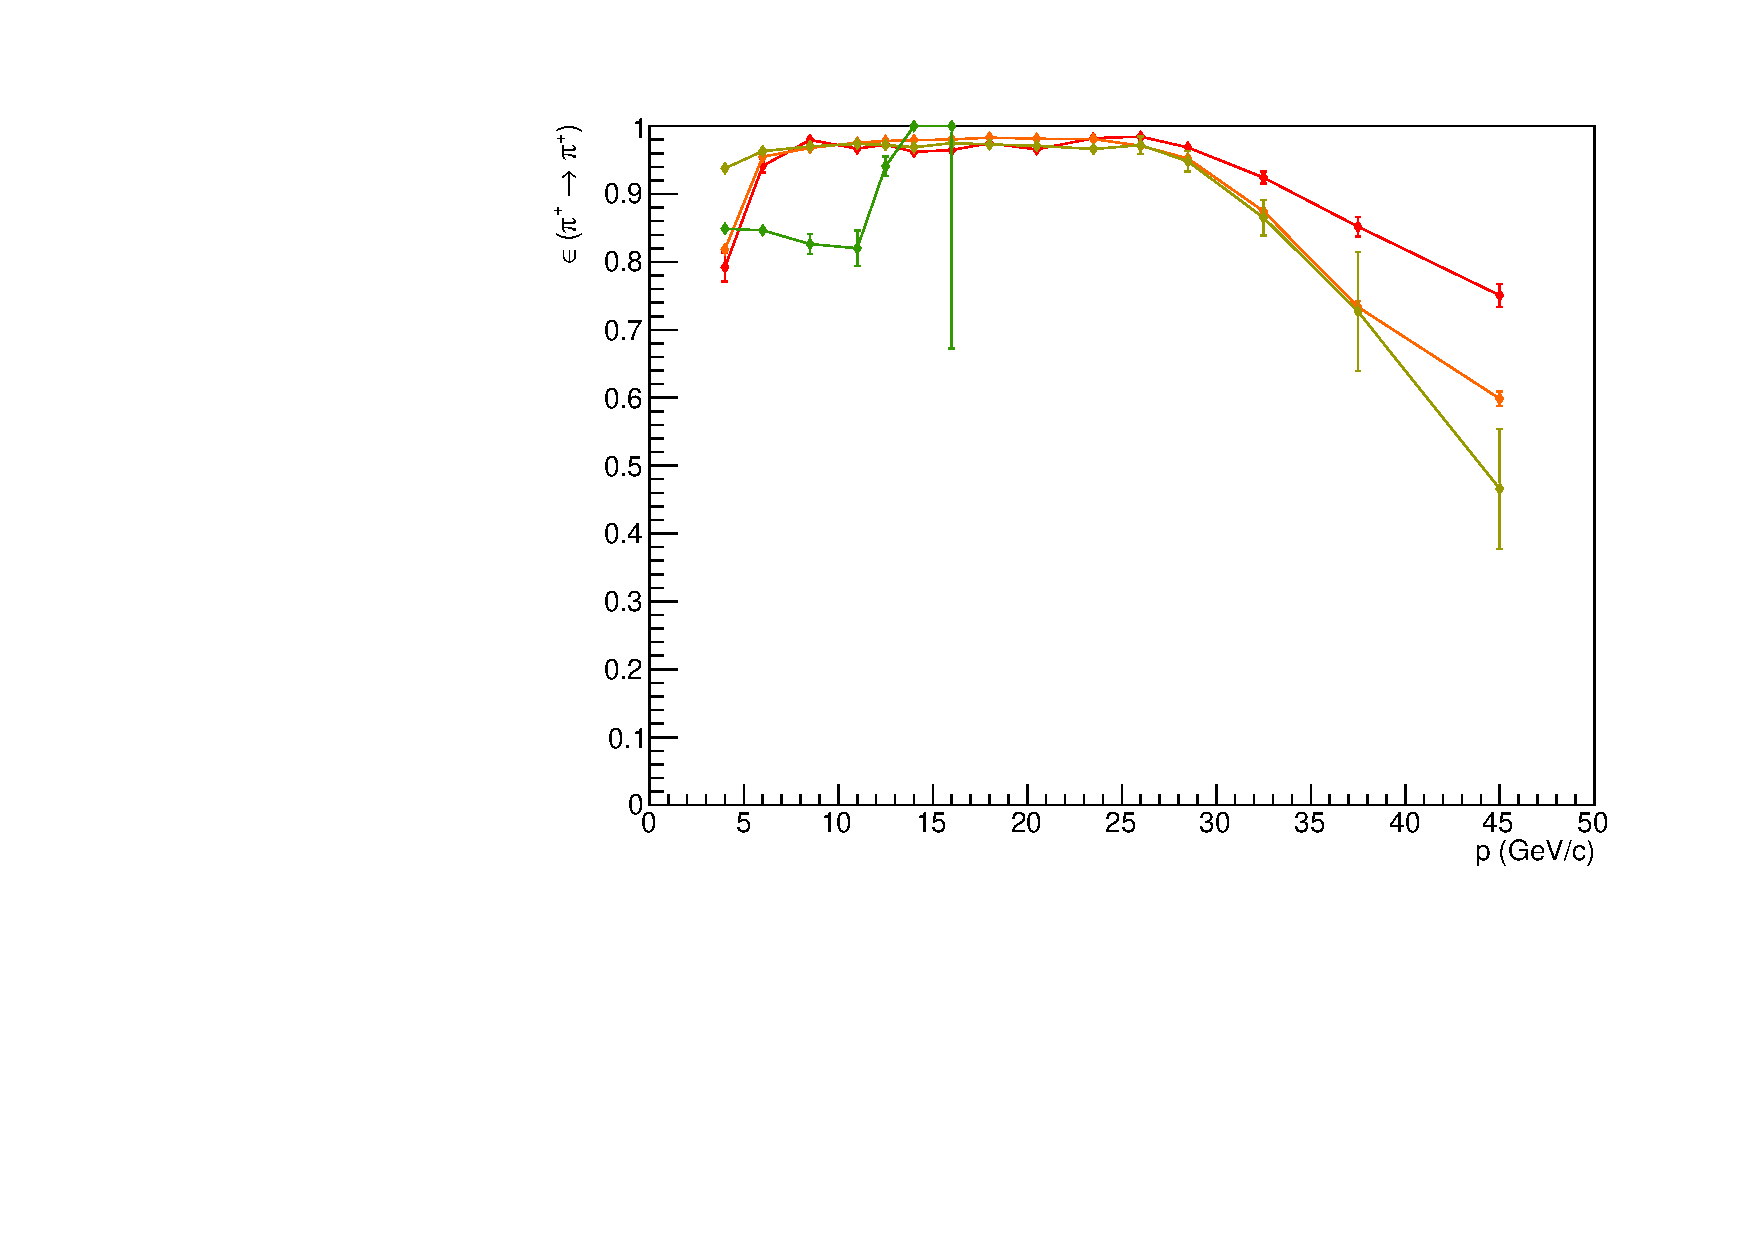
\includegraphics[scale=0.35]{./gfx/pip_pi.pdf}
  \includegraphics[scale=0.35]{./gfx/pip_K.pdf}
  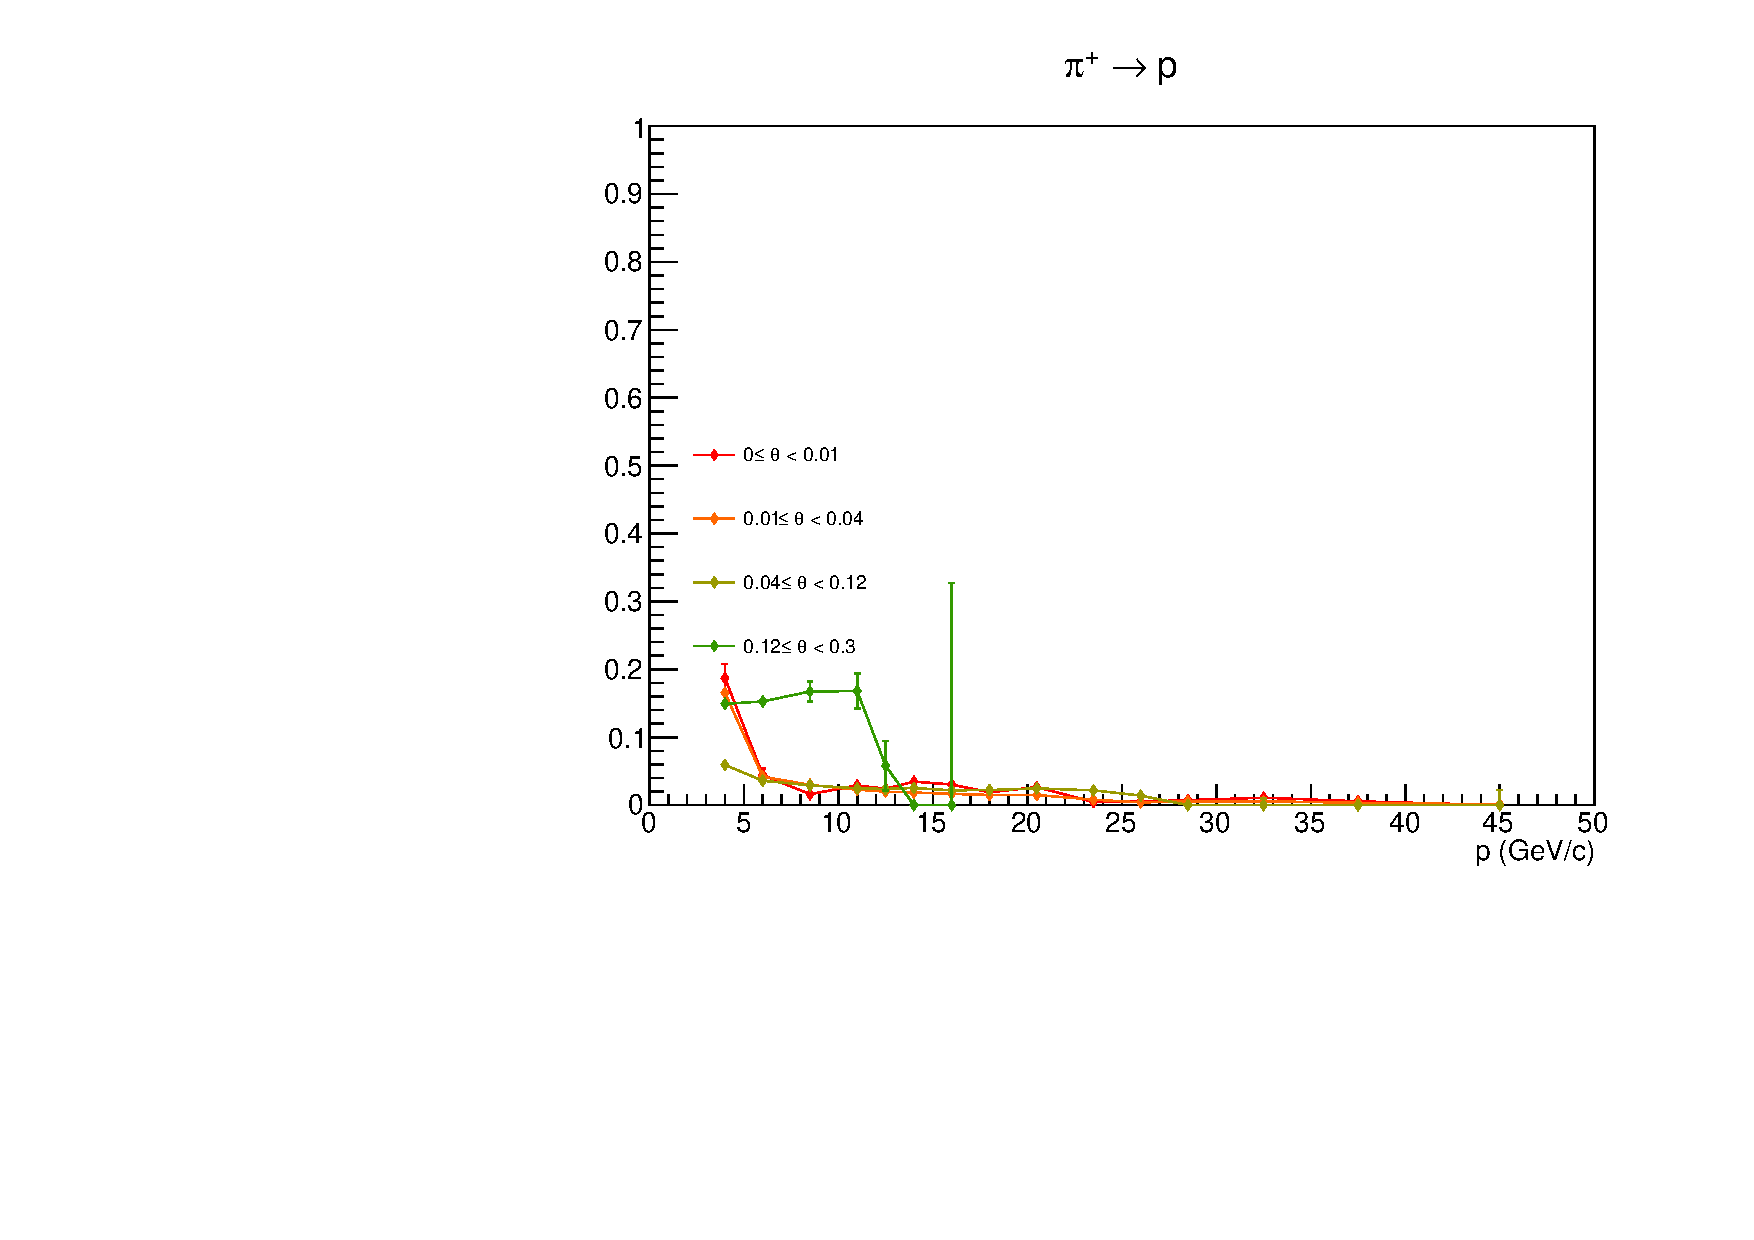
\includegraphics[scale=0.35]{./gfx/pip_p.pdf}
  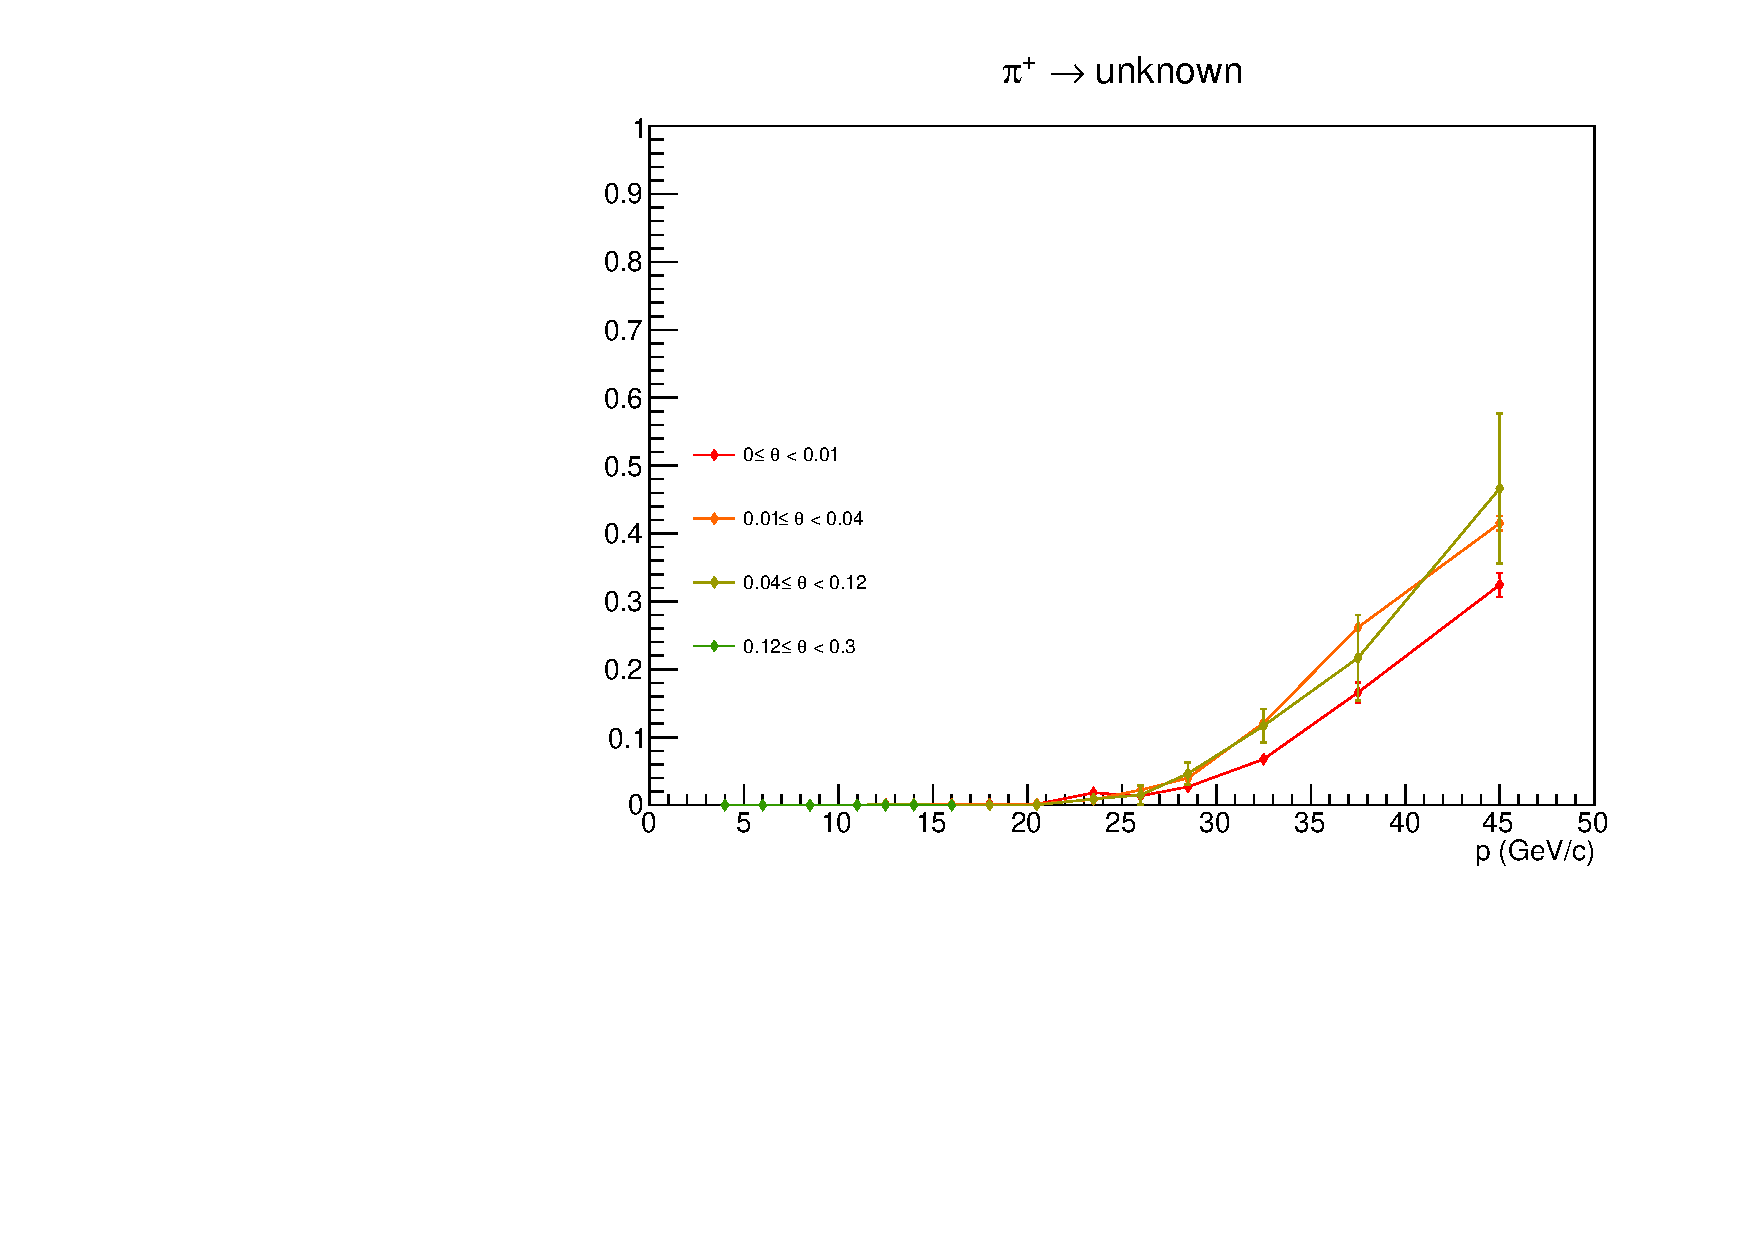
\includegraphics[scale=0.35]{./gfx/pip_u.pdf}
	\caption{Identification probabilities $\epsilon(p \rightarrow j)$ for $\pi^+$.}
	\label{pic:Effpip}
\end{figure}

\begin{figure}[!p]
  \centering
	\includegraphics[scale=0.35]{./gfx/Kp_pi.pdf}
  \includegraphics[scale=0.35]{./gfx/Kp_K.pdf}
  \includegraphics[scale=0.35]{./gfx/Kp_p.pdf}
  \includegraphics[scale=0.35]{./gfx/Kp_u.pdf}
	\caption{Identification probabilities $\epsilon(p \rightarrow j)$ for $K^+$.}
	\label{pic:Effkp}
\end{figure}

\newpage

\section{Problem at high $z$}

At some point it was discovered that at high momenta and high $z$ ($35$ GeV/$c$ < $p_h$ < $40$ GeV/$c$, $z$ > $0.7$), a contamination of the kaon sample by misidentified pions was observed, which was not accounted for in the efficiency matrix (Fig.~\ref{pic:NonLin}). Instead of the expected separation between pions and kaons at $LH_{\pi} = LH_K$, pions are found at $LH_{\pi} < LH_K$. We are now not looking at the clean samples but back to the normal data.

\begin{figure}[!h]
  \centering
	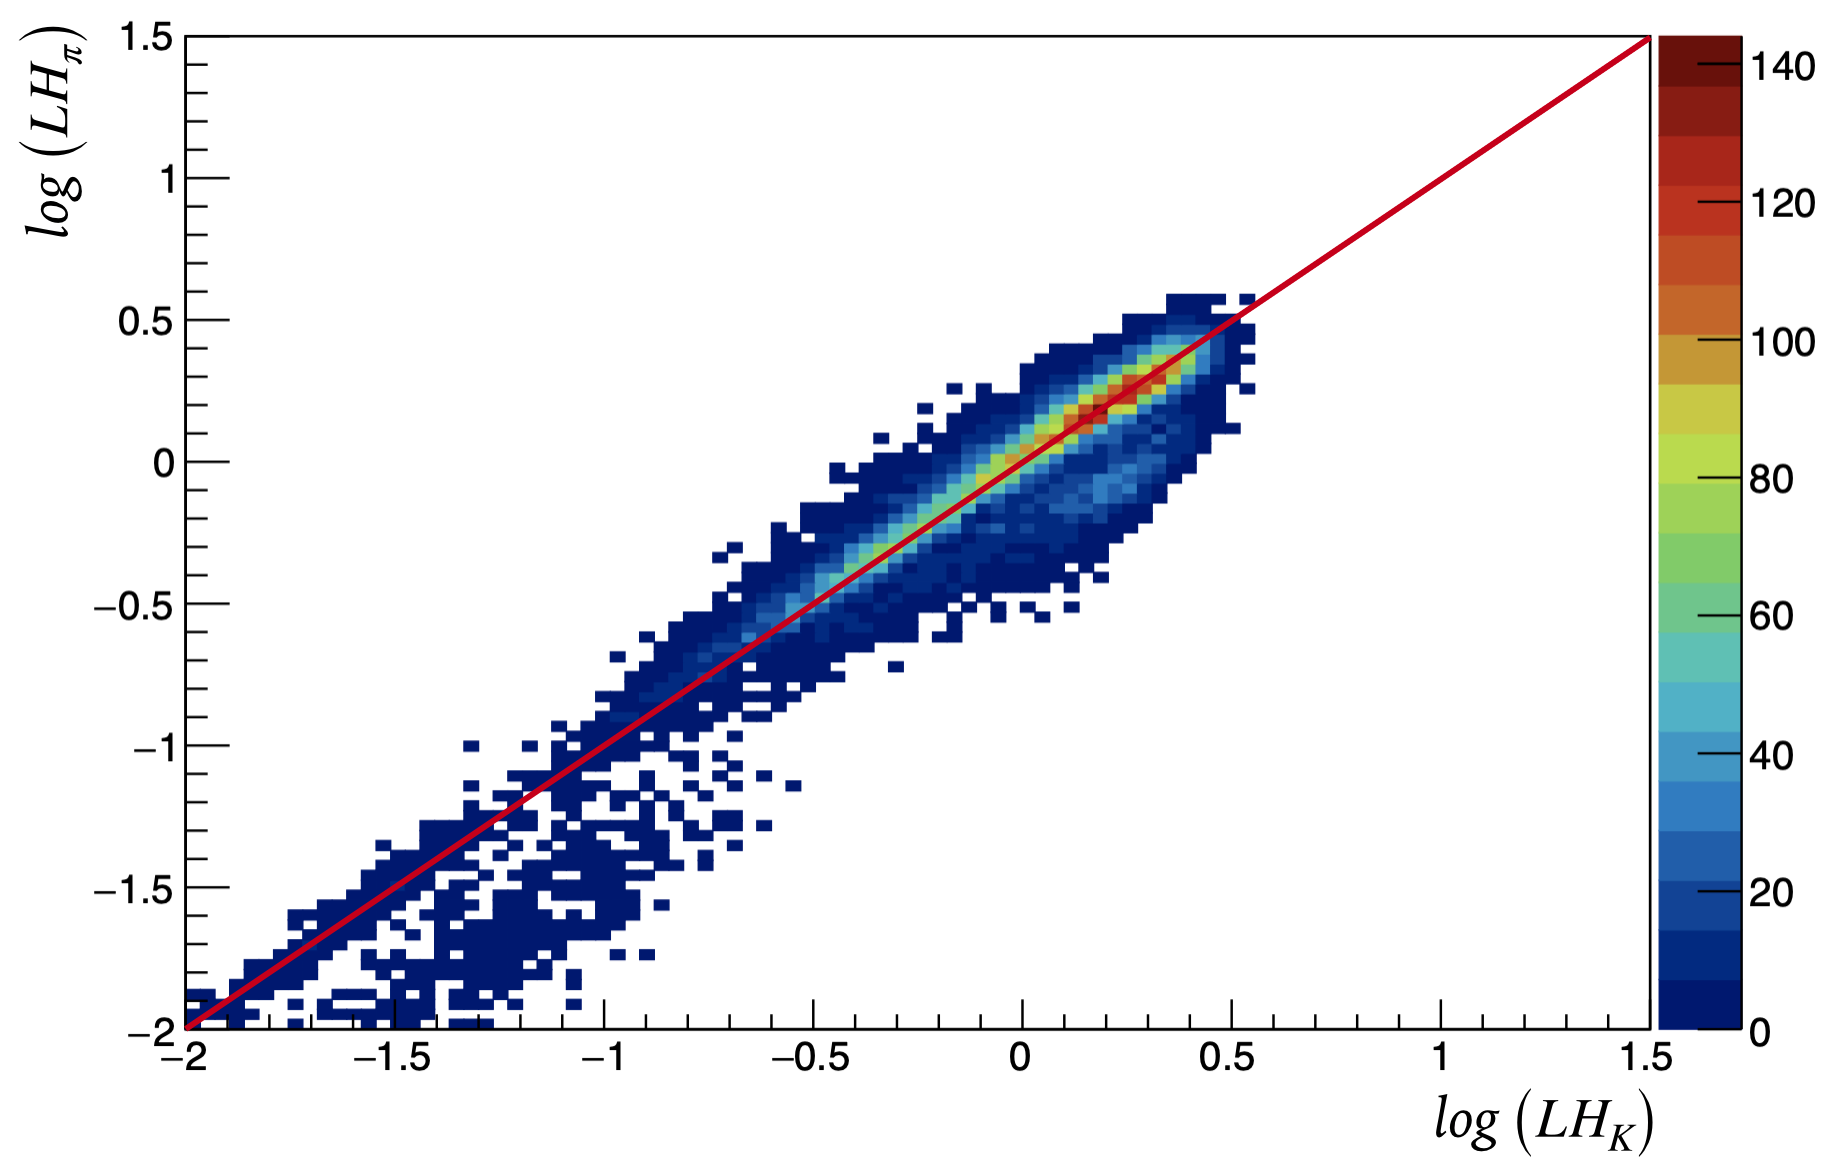
\includegraphics[scale=0.35]{./gfx/RICHLH.png}
	\caption{Likelihood for pions as a function of the likelihood for kaons using 2016 data.}
	\label{pic:NonLin}
\end{figure}

The larger the likelihood values are, the larger the effect is. This behaviour is also present in $2006$, $2007$ and $2011$ data (Fig. \ref{pic:NonLinother}). When investigating, it was shown that the probability for the misidentification of pions as kaons differs from the value given in the RICH tables in this kinematic region using the $p_T$ spectra \cite{MarcinNote}.

\begin{figure}[!h]
  \centering
	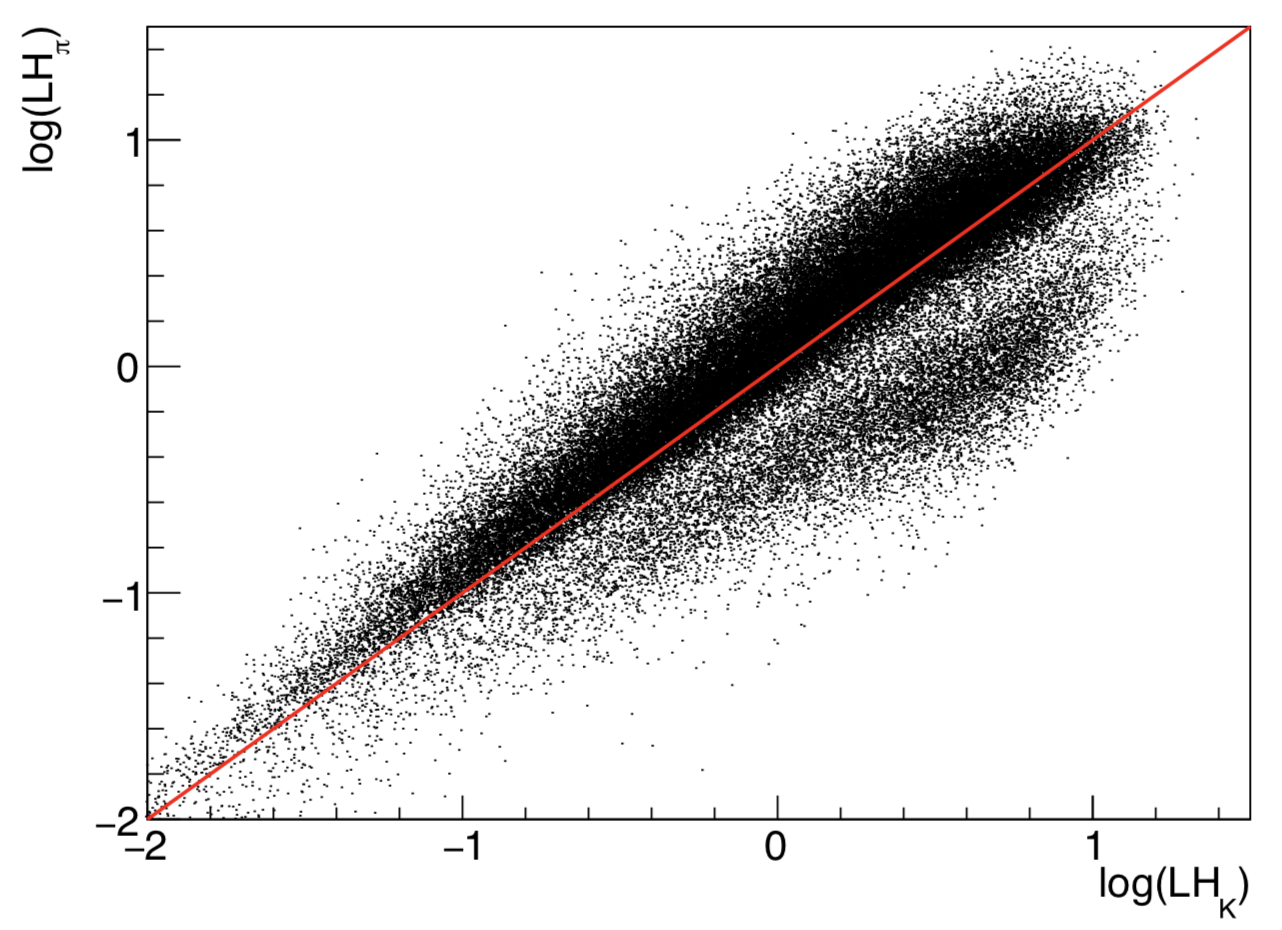
\includegraphics[scale=0.2]{./gfx/RICHLH2006.png}
  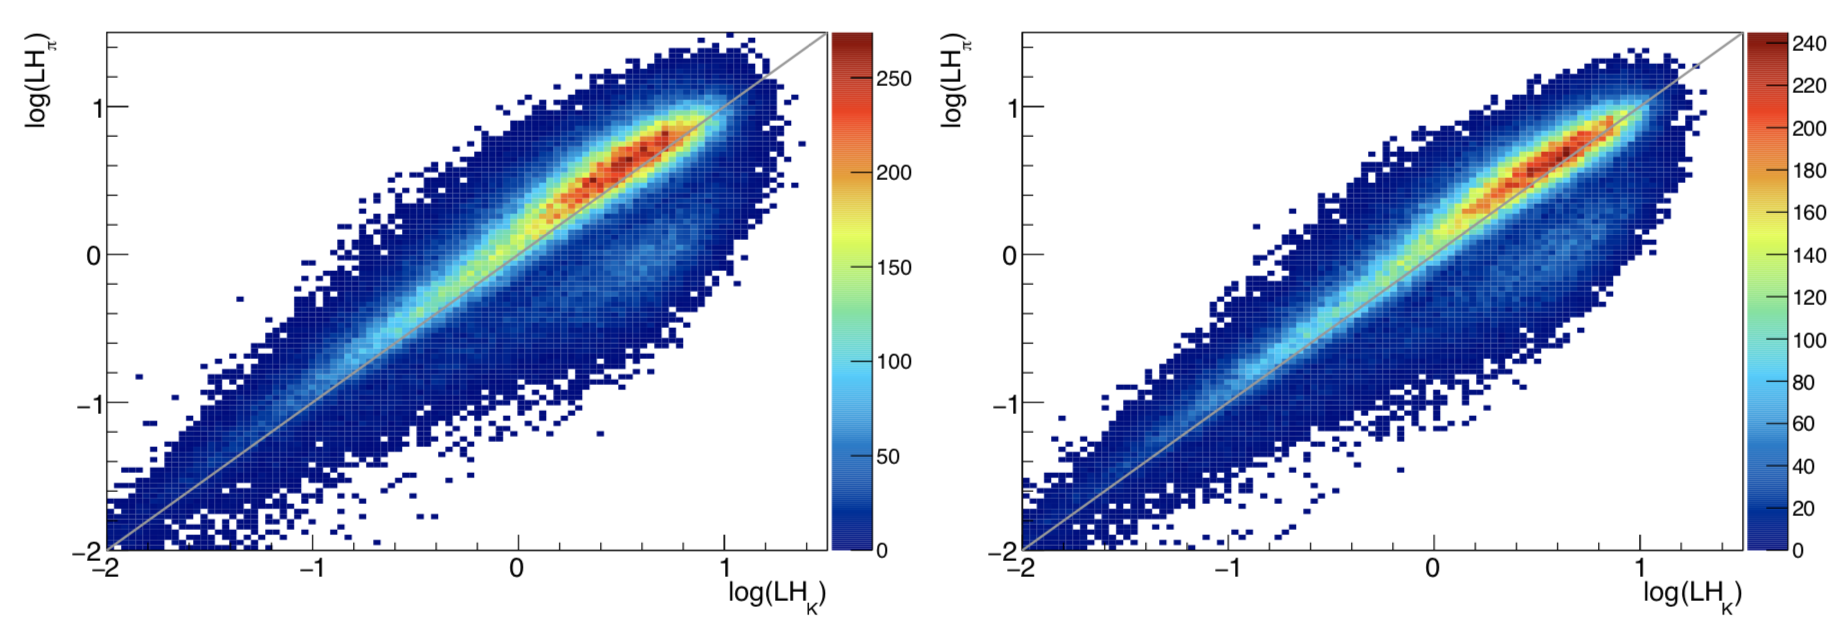
\includegraphics[scale=0.3]{./gfx/RICHLH2011.png}
	\caption{Likelihood for pions as a function of the likelihood for kaons using (from left to right) $2006$, $2007$ and $2011$ data.}
	\label{pic:NonLinother}
\end{figure}

In order to check if the non-linearities are taken correctly into account in the RICH tables, the likelihood values for pions and kaons are compared using the $K^0$ sample for high momenta and high $z$. This comparison is shown in Fig. \ref{pic:K0sample}, highlighting the fact that the problematic region is not covered by the $K^0$ sample and therefore the RICH table are not valid in this kinematic region.

\begin{figure}[!h]
  \centering
	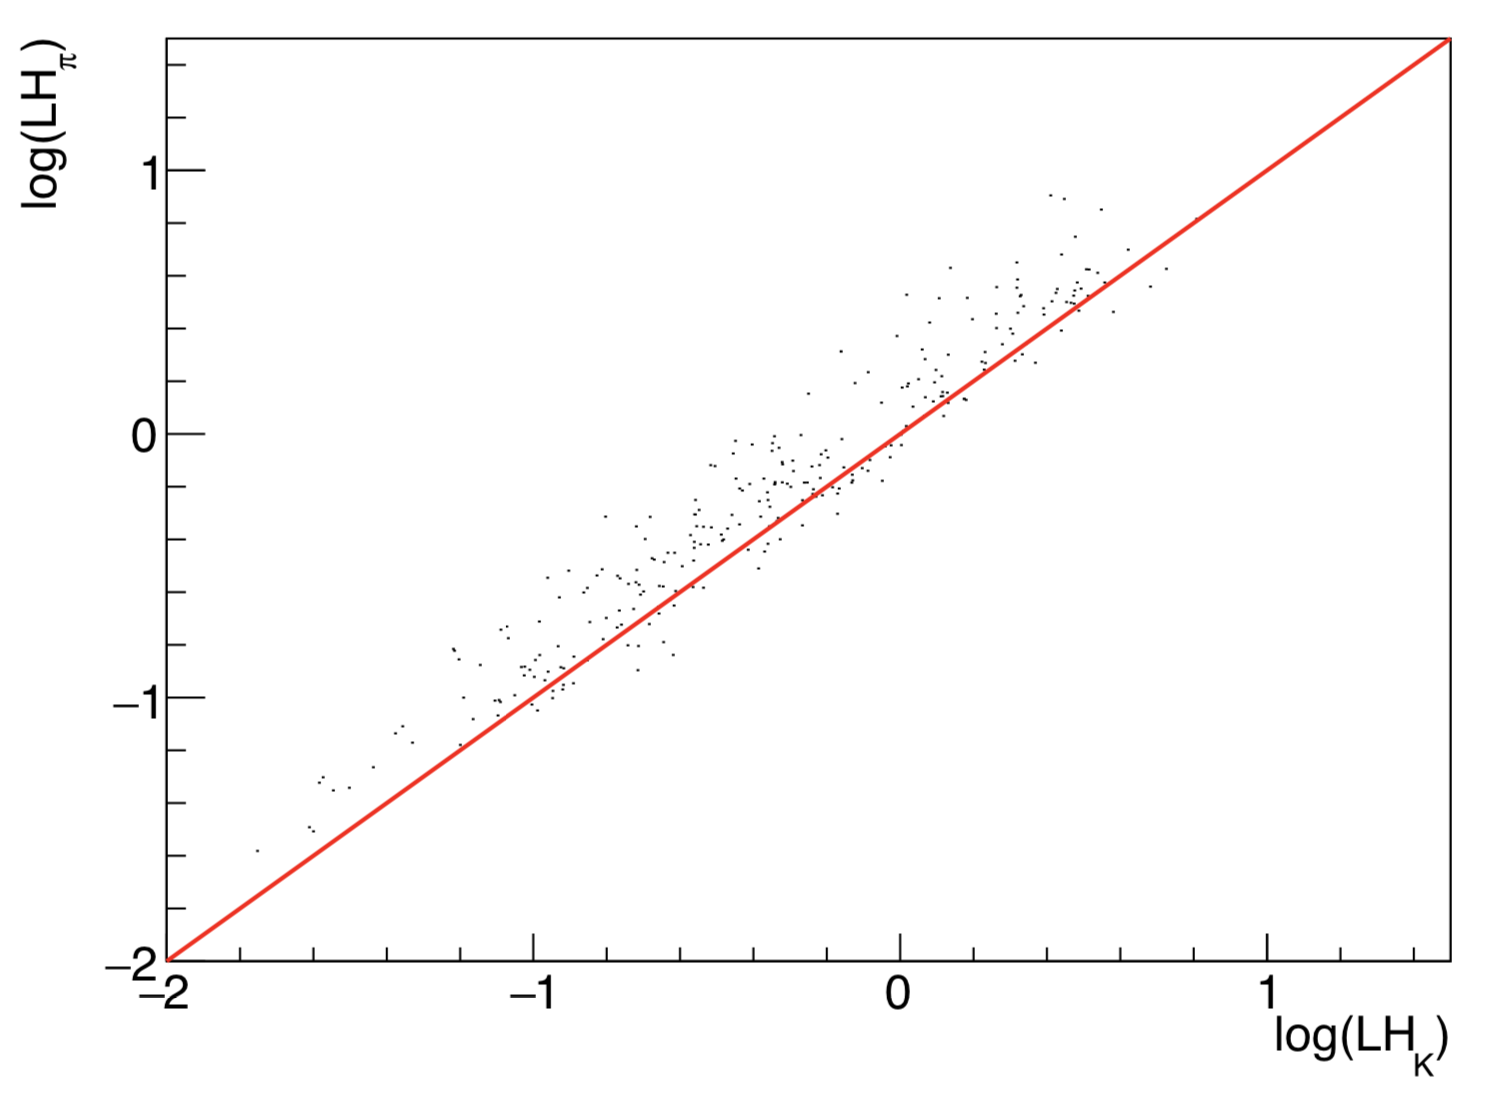
\includegraphics[scale=0.4]{./gfx/K0sample.png}
	\caption{Likelihood for pions as a function of the likelihood for kaons using the 2011 $K^0$ sample. Figure taken from \cite{RICHnote}.}
	\label{pic:K0sample}
\end{figure}

In order to obtain correct values for the RICH tables, a different sample for pions is needed. This new sample is obtained using the $\rho^0$ decay into two pions. The sample contains, in contrast to the $K^0$ sample, events at high momenta and high $z$, which covers high likelihood values. Though this method has been working for the $2006$ data it was not concluding with $2016$ data probably due to the lower statistics available for the current analysis compared to what was used in $2006$.

\begin{figure}[!h]
  \centering
	\subfloat[]{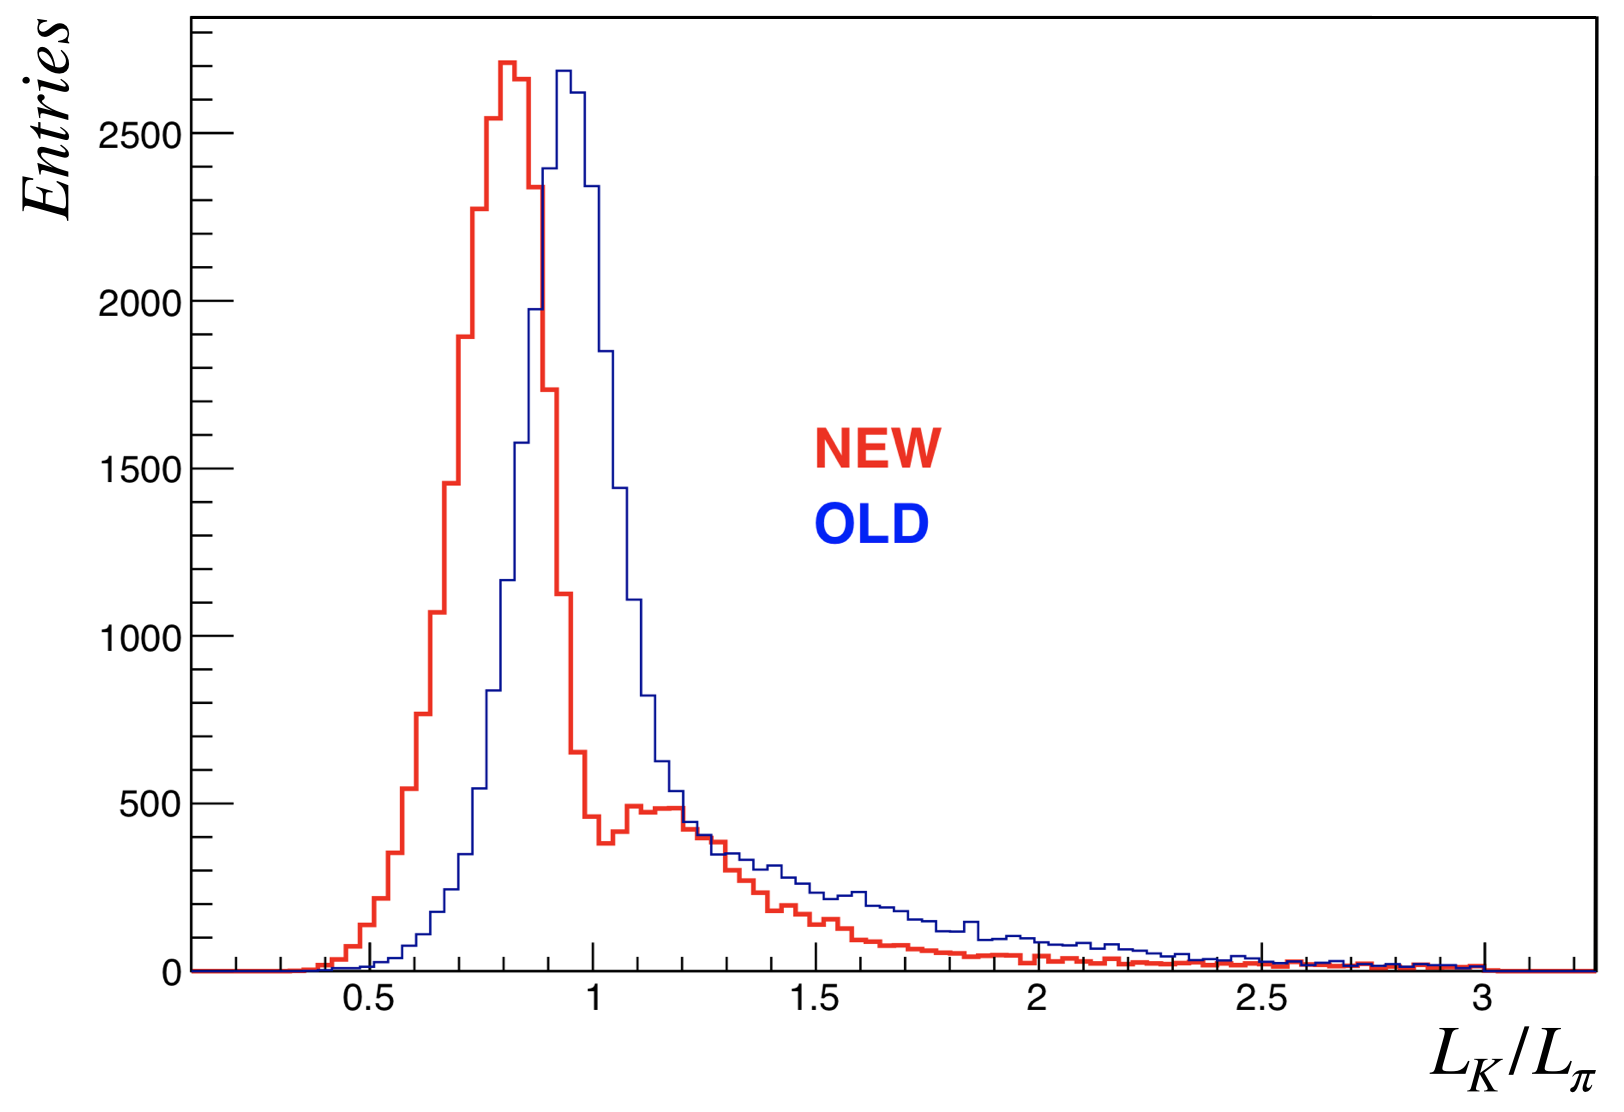
\includegraphics[scale=0.28]{./gfx/NewRICH1.png}}
  \subfloat[]{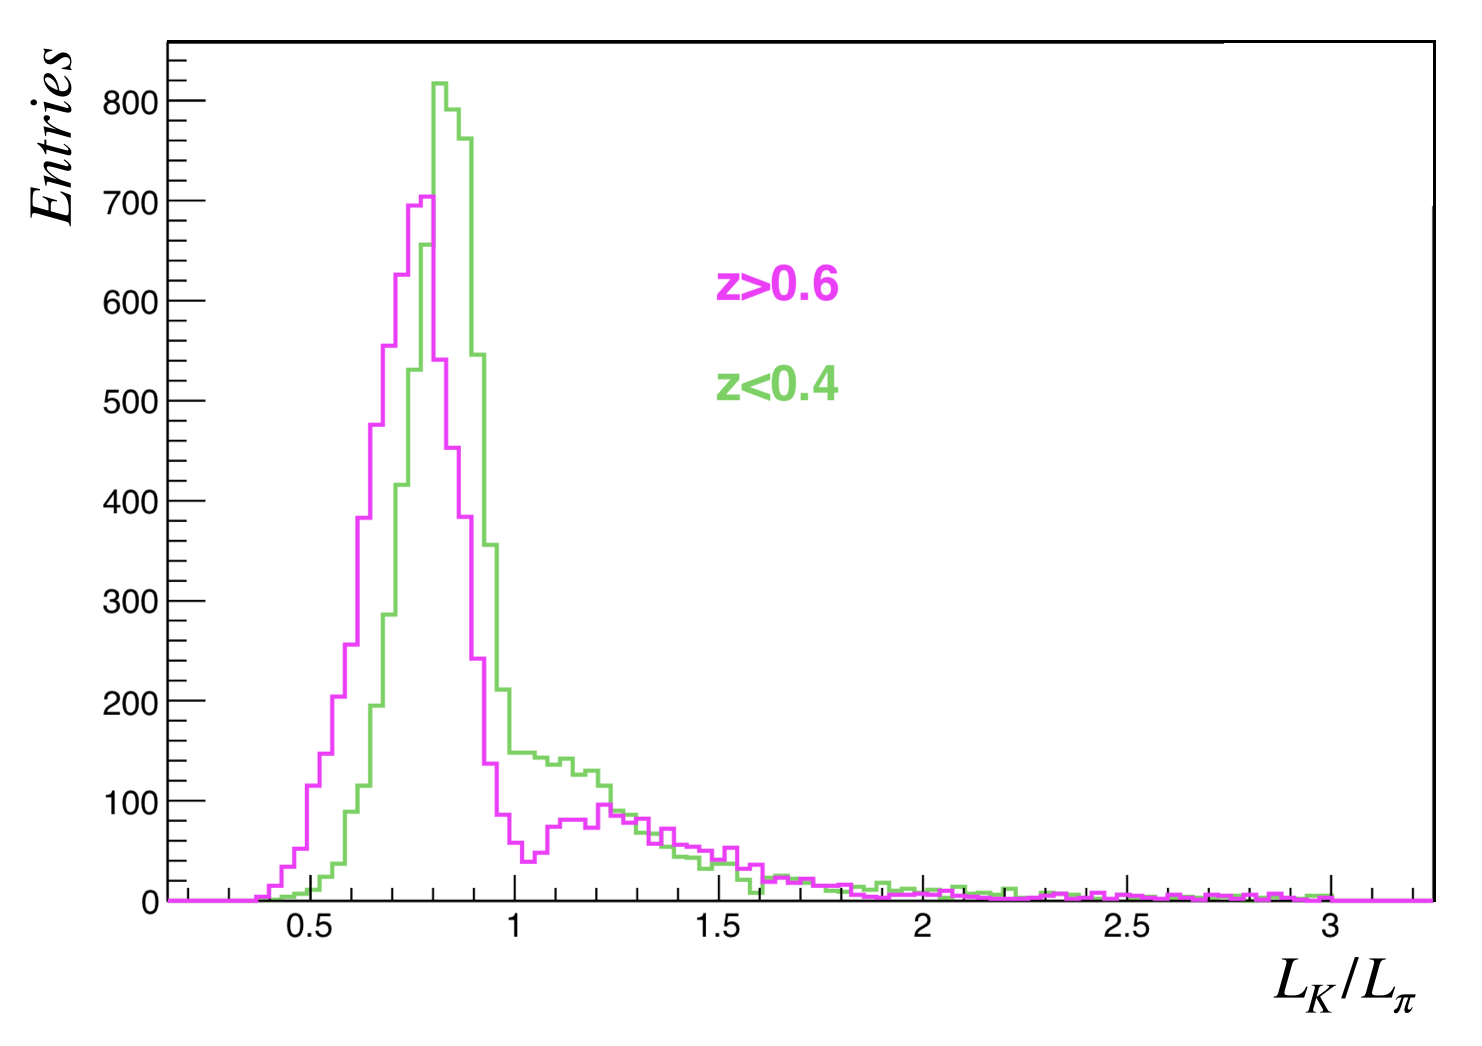
\includegraphics[scale=0.3]{./gfx/NewRICH2.png}}
	\caption{Figure (a) displays the likelihood ratio $L_{K}/L_{\pi}$ before (blue curve) and after (red curve) the new alignement of the RICH. The separation minimum is visible at $L_{K}/L_{\pi} = 1$ with the new alignement. Figure (b) compares the likelihood ratio $L_{K}/L_{\pi}$ for $z>0.6$ (magenta curve) and $z<0.4$ (green curve). While previously likelihoods were perfoming worse with $z$, the trend is as expected with the new alignement. Figures taken from \cite{MarcinNew}.}
	\label{pic:newRICH}
\end{figure}

These non-linearities have been adressed recently by the COMPASS RICH group. They have been reporting that the mirrors were not placed at the right place. A refinement of the alignement has an effect on the refractive index extraction and subsequently improving the pion versus kaon likelihoods picture, apparently curing the non-linearities. Further tests must still be done in order to quantify the improvement but preliminary studies \cite{MarcinNew} displayed in Fig.~\ref{pic:newRICH} show for the moment that the misidentification problem adressed in this section has been corrected. The $\pi$ peak is now below $L_{K}/L_{\pi} = 1$ and the separation minimum close to $L_{K}/L_{\pi} = 1$ is visible. In addition, while previously likelihoods were performing worse at high $z$, now the trend is as expected. This new alignement of the RICH has not been taken into account in the following analysis.

\section{Comparison of the efficiencies of 2006 to 2016}

In order to see if the RICH has been stable in terms of efficiency and purity through time, it is possible to compare the RICH efficiencies for $2006$, $2011$ and $2016$ (Fig. \ref{pic:comppip} to \ref{pic:comppm}). The first data taking with the refurbished RICH was done in $2006$. All these effiencies are extracted using the same likelihood cuts. The results point to a good stability of the RICH through time, even improving for some efficiencies, like pion identification for example. All data support the good identification of all species in the selected momentum range highlighting the excellent separation performed by the RICH.

\begin{figure}[!h]
  \centering
	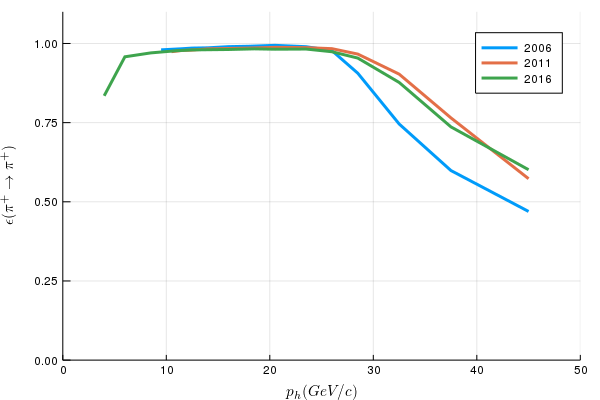
\includegraphics[scale=0.35]{./gfx/t1/pip2pip.png}
  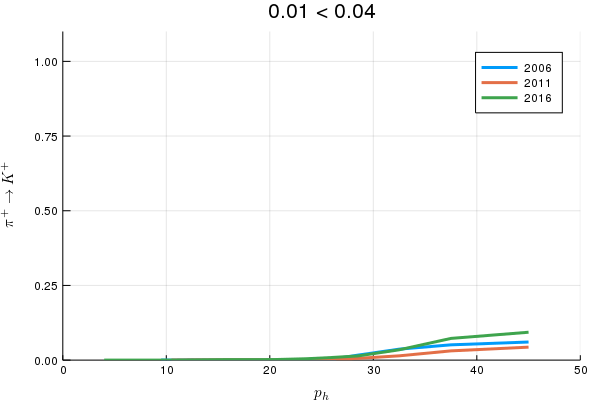
\includegraphics[scale=0.35]{./gfx/t1/pip2kp.png}
  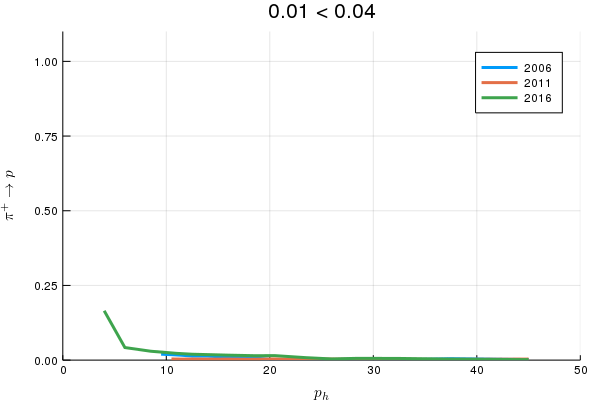
\includegraphics[scale=0.35]{./gfx/t1/pip2pp.png}
	\caption{Identification probabilities $\epsilon(p \rightarrow j)$ for $\pi^+$ in the bin $0.01$ rad $<$ $\theta$ $<$ $0.04$ rad for 3 different years : 2006 (blue), 2011 (orange) and 2016 (green).}
	\label{pic:comppip}
\end{figure}

\begin{figure}[!p]
  \centering
	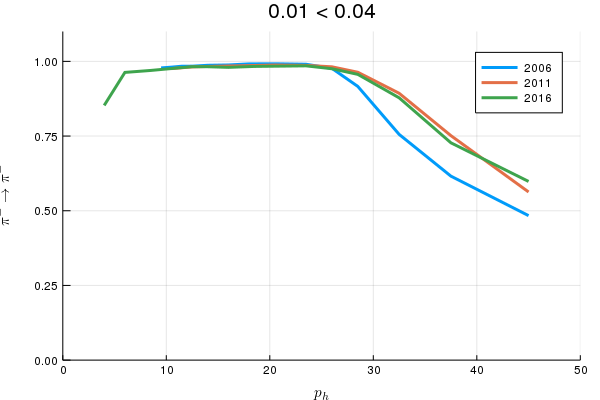
\includegraphics[scale=0.35]{./gfx/t1/pim2pim.png}
  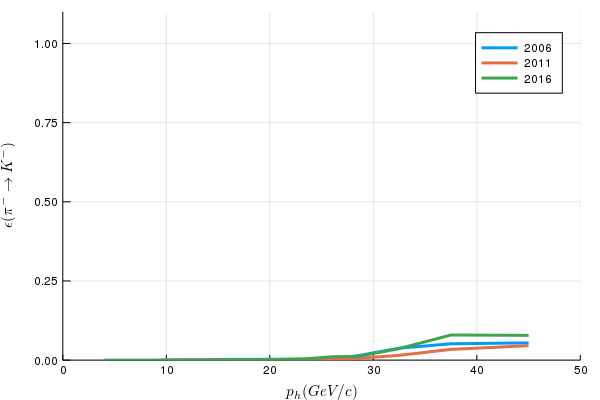
\includegraphics[scale=0.35]{./gfx/t1/pim2km.png}
  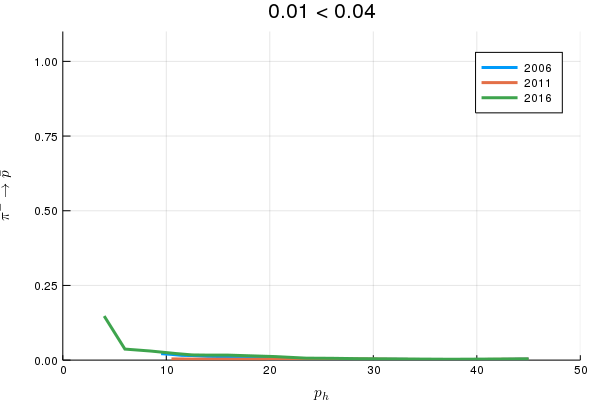
\includegraphics[scale=0.35]{./gfx/t1/pim2pm.png}
	\caption{Same as Fig.~\ref{pic:comppip} for $\epsilon(p \rightarrow j)$.}
	\label{pic:comppim}
\end{figure}

\begin{figure}[!p]
  \centering
	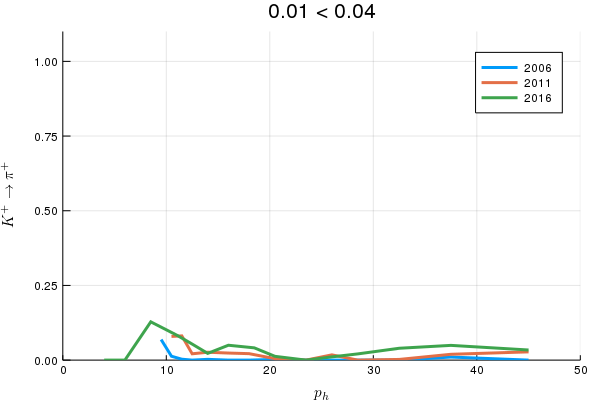
\includegraphics[scale=0.35]{./gfx/t1/kp2pip.png}
  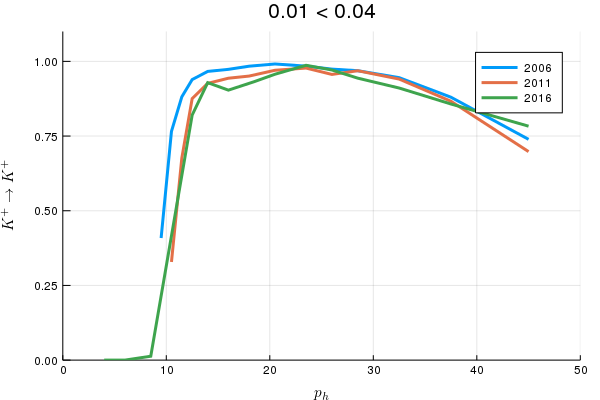
\includegraphics[scale=0.35]{./gfx/t1/kp2kp.png}
  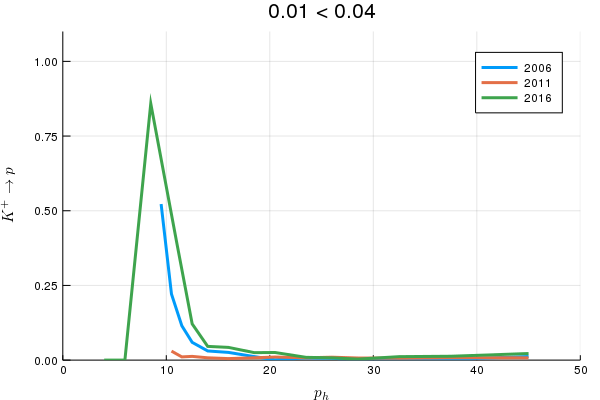
\includegraphics[scale=0.35]{./gfx/t1/kp2pp.png}
	\caption{Same as Fig.~\ref{pic:comppip} for $\epsilon(p \rightarrow j)$.}
	\label{pic:compkp}
\end{figure}

\begin{figure}[!p]
  \centering
	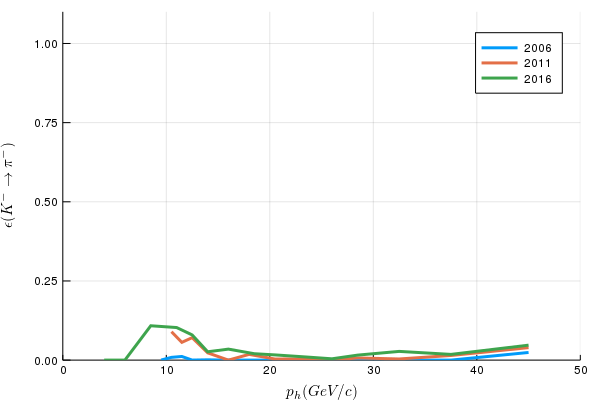
\includegraphics[scale=0.35]{./gfx/t1/km2pim.png}
  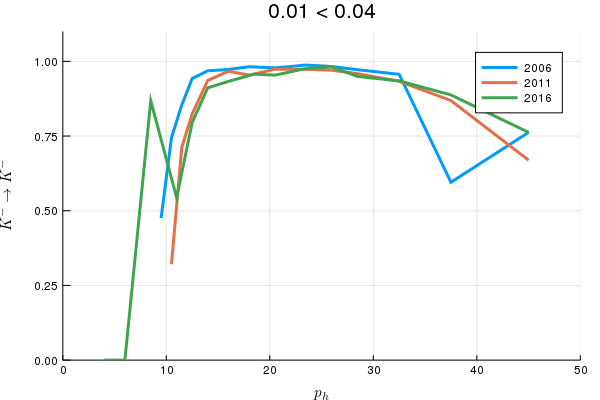
\includegraphics[scale=0.35]{./gfx/t1/km2km.png}
  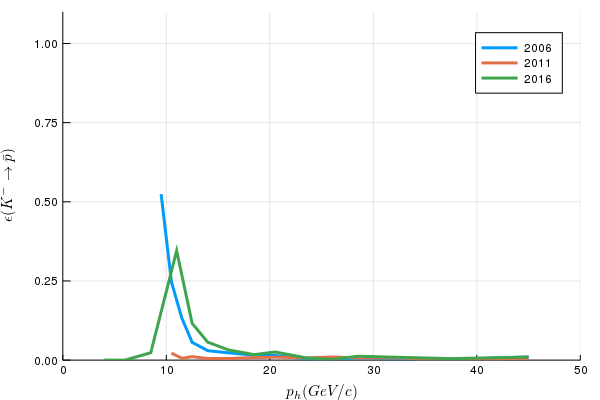
\includegraphics[scale=0.35]{./gfx/t1/km2pm.png}
	\caption{Same as Fig.~\ref{pic:comppip} for $\epsilon(p \rightarrow j)$.}
	\label{pic:compkm}
\end{figure}

\begin{figure}[!p]
  \centering
	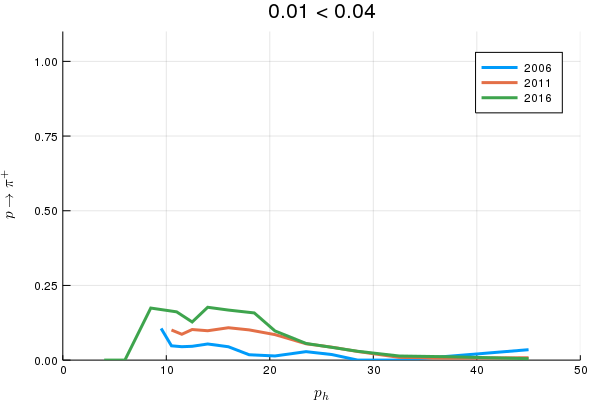
\includegraphics[scale=0.35]{./gfx/t1/pp2pip.png}
  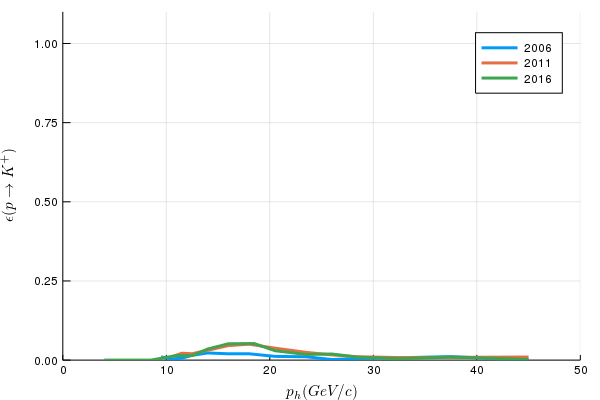
\includegraphics[scale=0.35]{./gfx/t1/pp2kp.png}
  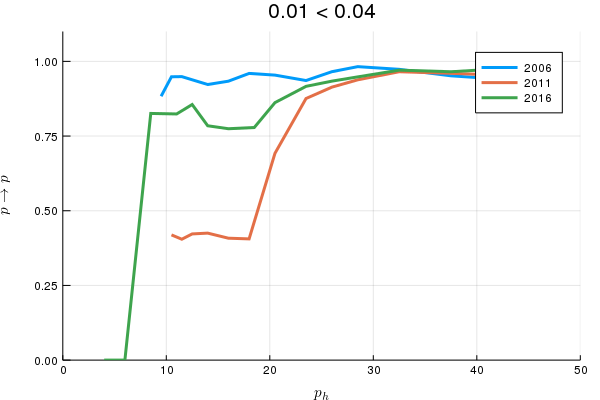
\includegraphics[scale=0.35]{./gfx/t1/pp2pp.png}
	\caption{Same as Fig.~\ref{pic:comppip} for $\epsilon(p \rightarrow j)$.}
	\label{pic:comppp}
\end{figure}

\begin{figure}[!h]
  \centering
	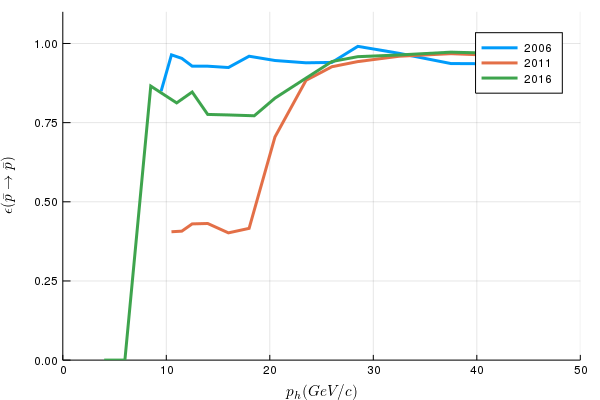
\includegraphics[scale=0.35]{./gfx/t1/pm2pm.png}
  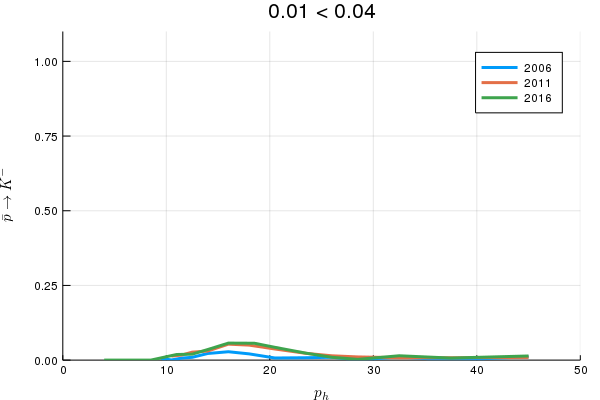
\includegraphics[scale=0.35]{./gfx/t1/pm2km.png}
  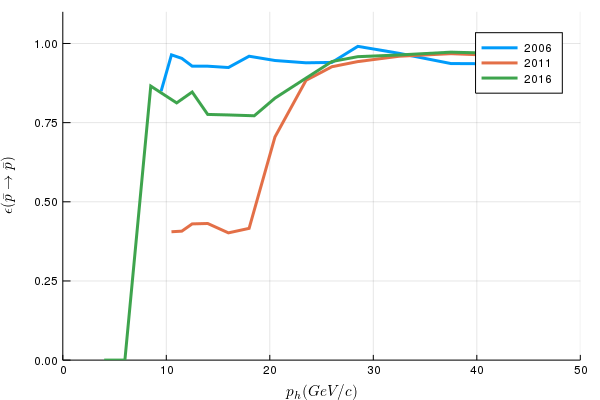
\includegraphics[scale=0.35]{./gfx/t1/pm2pm.png}
	\caption{Same as Fig.~\ref{pic:comppip} for $\epsilon(p \rightarrow j)$ for $\bar{p}$.}
	\label{pic:comppm}
\end{figure}

%----------------------------------------------------------------------------------------

\newpage

\section{Summary}

The RICH detector performances are determined from real data, using samples of $\pi$, $K$ and $p$ coming from the decay into two charged particles of $K^0$, $\Phi$ and $\Lambda$. In order to take into account the dependence of the RICH performance with the hadron phase-space, the performances are extracted in bins of the particle momentum $p_h$ and the track polar angle $\theta$ at the RICH entrance.

High identification probabilities are reached for $p_h$ below $30$ GeV/$c$. For pions, it reaches values larger than $97\%$ and for kaons and protons, it reaches values larger than $90\%$ except for the zones around the kaon and proton thresholds of $\sim$ $9.45$ and $\sim$ $17.95$ GeV/$c$, respectively. The identification probability values drop for larger $p_h$ values in the pion and kaon case due to the Cherenkov angle saturation ($\beta \rightarrow 1$). As a consequence, the misidentification probabilities are larger in this region.
